\documentclass{article}

\def\npart {II}
\def\nyear {2017}
\def\nterm {Lent}
\def\nlecturer{Dr R.\ Camina}
\def\ncourse{Coding and Cryptography}
\def\draft{Rough}
\ifx \nauthor\undefined
  \def\nauthor{Bhavik Mehta}
\else
\fi

\author{Based on lectures by \nlecturer \\\small Notes taken by \nauthor}
\date{\nterm\ \nyear}
\title{Part \npart\ -- \ncourse}

\usepackage[utf8]{inputenc}
\usepackage{amsmath}
\usepackage{amsthm}
\usepackage{amssymb}
\usepackage{enumerate}
\usepackage{mathtools}
\usepackage{graphicx}
\usepackage[dvipsnames]{xcolor}
\usepackage{tikz}
\usepackage{wrapfig}
\usepackage{centernot}
\usepackage{float}
\usepackage{braket}
\usepackage[hypcap=true]{caption}
\usepackage{enumitem}
\usepackage[colorlinks=true, linkcolor=mblue]{hyperref}
\usepackage[nameinlink,noabbrev]{cleveref}
\usepackage{nameref}
\usepackage[margin=1.5in]{geometry}

% Theorems
\theoremstyle{definition}
\newtheorem*{aim}{Aim}
\newtheorem*{axiom}{Axiom}
\newtheorem*{claim}{Claim}
\newtheorem*{cor}{Corollary}
\newtheorem*{conjecture}{Conjecture}
\newtheorem*{defi}{Definition}
\newtheorem*{eg}{Example}
\newtheorem*{ex}{Exercise}
\newtheorem*{fact}{Fact}
\newtheorem*{law}{Law}
\newtheorem*{lemma}{Lemma}
\newtheorem*{notation}{Notation}
\newtheorem*{prop}{Proposition}
\newtheorem*{question}{Question}
\newtheorem*{rrule}{Rule}
\newtheorem*{thm}{Theorem}
\newtheorem*{assumption}{Assumption}

\newtheorem*{remark}{Remark}
\newtheorem*{warning}{Warning}
\newtheorem*{exercise}{Exercise}

% \newcommand{\nthmautorefname}{Theorem}

\newtheorem{nthm}{Theorem}[section]
\newtheorem{nlemma}[nthm]{Lemma}
\newtheorem{nprop}[nthm]{Proposition}
\newtheorem{ncor}[nthm]{Corollary}
\newtheorem{ndef}[nthm]{Definition}

% Special sets
\newcommand{\C}{\mathbb{C}}
\newcommand{\N}{\mathbb{N}}
\newcommand{\Q}{\mathbb{Q}}
\newcommand{\R}{\mathbb{R}}
\newcommand{\Z}{\mathbb{Z}}

\newcommand{\abs}[1]{\left\lvert #1\right\rvert}
\newcommand{\norm}[1]{\left\lVert #1\right\rVert}
\renewcommand{\vec}[1]{\boldsymbol{\mathbf{#1}}}

\let\Im\relax
\let\Re\relax

\DeclareMathOperator{\Im}{Im}
\DeclareMathOperator{\Re}{Re}
\DeclareMathOperator{\id}{id}

\definecolor{mblue}{rgb}{0., 0.05, 0.6}


% preamble
\usepackage{tikz}
\usepackage{pgfplots}
\usepackage{tikz-cd}
\usepackage{extarrows}
\usepackage{bbm}
\usepackage{bm}
\usepackage{wrapfig}
\usepackage{xfrac}
\usetikzlibrary{arrows,decorations.pathmorphing,decorations.markings,positioning}
\DeclarePairedDelimiter{\floor}{\lfloor}{\rfloor}
\DeclarePairedDelimiter{\ceil}{\lceil}{\rceil}
\pgfplotsset{width=7cm}
\newcommand{\barP}{\mid}
\newcommand{\probConv}{\hyperlink{def:probConverge}{\xlongrightarrow{p}}}
\newcommand{\Prob}{\mathbb{P}}
\newcommand{\Exp}{\mathbb{E}}
\newcommand{\F}{\mathbb{F}}
\newcommand{\1}[1]{\mathbbm{1}_{#1}}
\DeclareMathOperator{\rank}{rank}
\DeclareMathOperator{\RM}{RM}
\DeclareMathOperator{\ord}{ord}
% and here we go!

\begin{document}
\maketitle
\tableofcontents

\clearpage
\section*{Introduction to communication channels and coding}
For example, given a message $m$=`Call me!' which we wish to send by email, first encode as binary strings using ASCII.
So, $f(C) = 1000011, f(a) = 1100001$, and $f^*(m) = 1000011\ 1100001 \dots 0100001$.
\tikzstyle{block} = [rectangle, draw, fill=YellowOrange!20,
    text width=4em,
    text centered,
    minimum height=2em
    ]
\begin{center}
    \begin{tikzpicture}[node distance=3cm]
        \node (s) at (0, 0) [block] {source};
        % this is kind of horrible but it works :/
        \node (e) at (3, 0) [block] {encoder};
        \node (d) at (8, 0) [block] {decoder};
        \node (r) at (11, 0) [block] {receiver};
        \draw [->, shorten > =0.1em, thick] (s) -- (e);
        \draw [->, shorten > =0.1em, thick, decorate, decoration={amplitude=1.5mm,
            segment length=10mm,
            snake, post length=1mm}] (e) -- (d)
            node [above=0.5em,align=center,midway] {channel}
            node [below=0.5em,align=center,midway,color=red] {errors};

        \draw [->, shorten > =0.1em, thick] (d) -- (r);
    \end{tikzpicture}
\end{center}

\textbf{Basic problem:} Given a source and a channel (described probabilistically) we aim to design an encoder and a decoder in order to transmit information both \emph{economically} and \emph{reliably} (coding) and maybe also to \emph{preserve privacy} (cryptography).

\begin{eg}
\leavevmode
\begin{itemize}[label={--}]
    \item `Economically': In Morse code, common letters have shorter codewords:
    \begin{equation*}
        A = \text{.-} \quad E = \text{.} \quad Q = \text{-{}-.-}
    \end{equation*}
    \item `Reliably': Every book has an ISBN of form $a_1 a_2 \dotsc a_{10}$ where $a_i \in \{0, 1, \dotsc, 9\}$ for $1 \leq i \leq 9$, $a_{10} \in \{0, 1, \dotsc, 9, X\}$ such that
    \begin{equation*}
        10 a_1 + 9 a_2 + \dotsc + a_{10} \equiv 0 \pmod{11}
    \end{equation*}
    so errors can be detected (but not corrected).
    Similarly a 13-digit ISBN has
    \begin{equation*}
        x_1 + 3 x_2 + x_3 + 3 x_4 + \dotsc + 3 x_{12} + x_{13} \equiv 0 \pmod{10}
    \end{equation*}
    for $0 \leq x_i \leq 10$, doesn't necessarily spot transpositions.
    \item `Preserve privacy' e.g. RSA.
\end{itemize}
\end{eg}

A \textbf{communication channel} takes letters from an input alphabet $\Sigma_1 = \{a_1, \dotsc, a_r\}$ and emits letters form an output alphabet $\Sigma_2 = \{b_1, \dotsc, b_s\}$.

A channel is determined by the probabilities
\begin{equation*}
    \Prob(y_1 \dotsc y_k \text{ received} \mid x_1 \dotsc x_k \text{ sent})
\end{equation*}

\begin{defi}[Discrete memoryless channel]\hypertarget{def:dmc}
    A \textbf{discrete memoryless channel} (DMC) is a channel for which
    \begin{equation*}
        P_{ij} = \Prob(b_j \text{ received} \mid a_i \text{ sent})
    \end{equation*}
    is the same each time the channel is used and is independent of all past and future uses.
\end{defi}

The channel matrix is the $r \times s$ matrix with entries $p_{ij}$ (note the rows sum to 1).

\begin{eg}
    Binary Symmetric Channel \hypertarget{def:bsc}{(BSC)} has $\Sigma_1 = \Sigma_2 = \{0, 1\}$, $0 \leq p \leq 1$:
    \begin{center}
        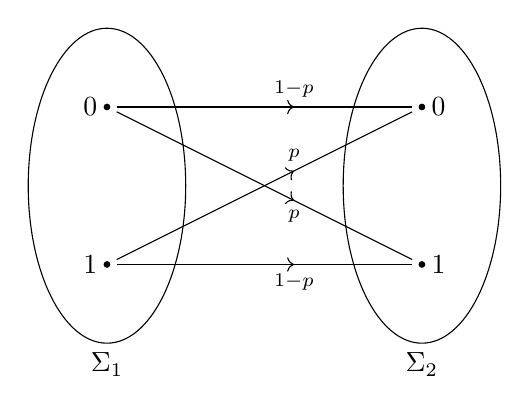
\begin{tikzpicture}
            \draw (-2, 0) circle [x radius=1cm, y radius=2cm] node [below=2cm] {$\Sigma_1$};
            \draw ( 2, 0) circle [x radius=1cm, y radius=2cm] node [below=2cm] {$\Sigma_2$};

            \node (0l) at (-2, 1) {};
            \node (1l) at (-2,-1) {};

            \node (0r) at (2, 1) {};
            \node (1r) at (2,-1) {};

            \filldraw (0l) circle (1pt) node [left] {0};
            \filldraw (1l) circle (1pt) node [left] {1};
            \filldraw (0r) circle (1pt) node [right] {0};
            \filldraw (1r) circle (1pt) node [right] {1};

            \begin{scope}[decoration={
                markings,
                mark=at position 0.6 with {\arrow{>}}}
                ]
                \draw[postaction={decorate}] (0l) -- (0r)
                    node [above,align=center,pos=0.6] {$\scriptstyle 1-p$};
                \draw[postaction={decorate}] (0l) -- (1r)
                    node [below,align=center,pos=0.6] {$\scriptstyle p$};
                \draw[postaction={decorate}] (1l) -- (0r)
                    node [above,align=center,pos=0.6] {$\scriptstyle p$};
                \draw[postaction={decorate}] (1l) -- (1r)
                    node [below,align=center,pos=0.6] {$\scriptstyle 1-p$};
            \end{scope}
        \end{tikzpicture}
    \end{center}
    with channel matrix
    \begin{equation*}
        \begin{pmatrix}
            1-p & p \\ p & 1-p
        \end{pmatrix}
    \end{equation*}
    i.e. $p$ is the probability a symbol is mistransmitted.


    Another example is given by the Binary Erasure channel, $\Sigma_1 \{0, 1\}$, $\Sigma_2 = \{0, 1, *\}$ and $0 \leq p \leq 1$.
    \begin{center}
        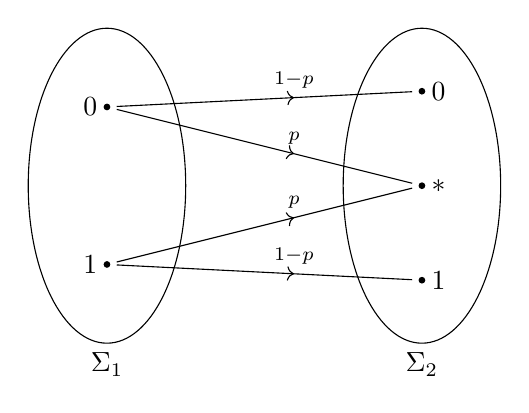
\begin{tikzpicture}
            \draw (-2, 0) circle [x radius=1cm, y radius=2cm] node [below=2cm] {$\Sigma_1$};
            \draw ( 2, 0) circle [x radius=1cm, y radius=2cm] node [below=2cm] {$\Sigma_2$};

            \node (0l) at (-2, 1) {};
            \node (1l) at (-2,-1) {};

            \node (0r) at (2, 1.2) {};
            \node (*r) at (2,   0) {};
            \node (1r) at (2,-1.2) {};

            \filldraw (0l) circle (1pt) node [left] {0};
            \filldraw (1l) circle (1pt) node [left] {1};
            \filldraw (0r) circle (1pt) node [right] {0};
            \filldraw (*r) circle (1pt) node [right] {$*$};
            \filldraw (1r) circle (1pt) node [right] {1};

            \begin{scope}[decoration={
                markings,
                mark=at position 0.6 with {\arrow{>}}}
                ]
                \draw[postaction={decorate}] (0l) -- (0r)
                    node [above,align=center,pos=0.6] {$\scriptstyle 1-p$};
                \draw[postaction={decorate}] (0l) -- (*r)
                    node [above,align=center,pos=0.6] {$\scriptstyle p$};
                \draw[postaction={decorate}] (1l) -- (*r)
                    node [above,align=center,pos=0.6] {$\scriptstyle p$};
                \draw[postaction={decorate}] (1l) -- (1r)
                    node [above,align=center,pos=0.6] {$\scriptstyle 1-p$};
            \end{scope}
        \end{tikzpicture}
    \end{center}
    with channel matrix
    \begin{equation*}
        \begin{pmatrix}
            1-p & p & 0 \\
            0 & p & 1-p
        \end{pmatrix}
    \end{equation*}
    i.e. $p$ is the probability a symbol can't be read.
\end{eg}

Informally, a channel's capacity is the highest rate at which information can be reliably transmitted over the channel.
Rate refers to units of information per unit time, which we want to be high. Similarly, reliably means we want an arbitrarily small error probability.

\clearpage
\section{Noiseless Coding}
\begin{notation}
    For $\Sigma$ an alphabet, let $\Sigma^* = \bigcup_{n \geq 0} \Sigma^n$ be the set of all finite strings of elements of $\Sigma$.
\end{notation}
If $x = x_1 \dotsc x_r$, $y = y_1 \dotsc y_s$ are strings from $\Sigma$, write $xy$ for the concatenation $x_1 \dotsc x_r y_1 \dotsc y_s$.
Further, $\abs{x_1 \dotsc x_r y_1 \dotsc y_s} = r+s$, the length of the string.
\begin{defi}[Code]\hypertarget{def:code}
    Let $\Sigma_1, \Sigma_2$ be two alphabets. A \textbf{code} is a function $f: \Sigma_1 \to \Sigma_2^*$. The strings $f(x)$ for $x \in \Sigma_1$ are called \textbf{codewords}.
\end{defi}
\begin{eg}
    \leavevmode
    \begin{enumerate}[label=\arabic*)]
        \item
            \hypertarget{ex:greekFire}{Greek fire} \hyperlink{def:code}{code}:
            \begin{align*}
                \Sigma_1 &= \{\alpha, \beta, \gamma, \dotsc, \omega\} \quad \text{ 24 letters} \\
                \Sigma_2 &= \{1, 2, 3, 4, 5\}
            \end{align*}
            so, $\alpha \mapsto 11, \beta \mapsto 12, \dotsc, \omega \mapsto 54$.
        \item
            $\Sigma_1 = $ \{all words in the dictionary\}, and $\Sigma_2 = \{A, B, \dotsc, Z, [space]\}$
            and $f$=`spell the word and a space'\hypertarget{ex:comma-code}.
    \end{enumerate}
\end{eg}
Send a message $x_1 \dotsm x_n \in \Sigma_1^*$ as $f(x_1) \dotsm f(x_n) \in \Sigma_2^*$ i.e. extend $f$ to $f^*:\Sigma_1^* \to \Sigma_2^*$\hypertarget{def:fstar}{.}

\begin{defi}[Decipherable]\hypertarget{def:decipherable}
    A \hyperlink{def:code}{code} $f$ is \textbf{decipherable} if \hyperlink{def:fstar}{$f^*$} is injective, i.e. every string from $\Sigma_2^*$ arises from at most one message.
    Clearly we need $f$ injective, but this is not enough.
\end{defi}

% Lecture 2

\begin{eg}
    Take $\Sigma_1 = \{1, 2, 3, 4\}$, $\Sigma_2 = \{0, 1\}$ with
    \begin{equation*}
        f(1) = 0, f(2) = 1, f(3) = 00, f(4) = 01.
    \end{equation*}
    $f$ injective but $\hyperlink{def:fstar}{f^*}(312) = 0001 = f^*(114)$ so $f^*$ not \hyperlink{def:decipherable}{decipherable}.
\end{eg}

\begin{notation}
    \hypertarget{def:aary}{If} $\abs{\Sigma_1} = m$, $\abs{\Sigma_2} = a$, then we say $f$ is an $a$-ary code of size $m$. (If $a=2$ we say binary).
\end{notation}
\begin{aim}
    Construct \hyperlink{def:decipherable}{decipherable} \hyperlink{def:code}{codes} with short word lengths.
\end{aim}

Provided $f: \Sigma_1 \to \Sigma_2^*$ is injective, the following codes are always decipherable.
\begin{enumerate}[label=(\roman*)]
    \item A \textbf{block code} is a code with all codewords of the same length (e.g. \hyperlink{eg:greekFire}{Greek fire code}).
    \item In a \textbf{comma code}, we reserve one letter from $\Sigma_2$ that is only used to signal the end of the codeword (e.g. \hyperlink{ex:comma-code}{Example 2 above}).
    \item A \hypertarget{def:prefixFreeCode}{\textbf{prefix-free code}} is a code where no codeword is a prefix of another (if $x, y \in \Sigma_2^*$, $x$ is a prefix of $y$ if $y=xz$ for some $z \in \Sigma_2^*$.)
\end{enumerate}

\begin{remark}(i) and (ii) are special cases of (iii).
\end{remark}

\hyperlink{def:prefixFreeCode}{Prefix-free codes} are also known as \textbf{instantaneous codes} (i.e. a word can be recognised as soon as it is complete) or \textbf{self-punctuating codes}.

% thm 1.1
\begin{nthm}[Kraft's inequality]\label{thm:kraft}
    Let $\abs{\Sigma_1} = m, \abs{\Sigma_2} = a$. A \hyperlink{def:prefixFreeCode}{prefix-free code} $f: \Sigma_1 \to \Sigma_2^*$ with word lengths $s_1, \dotsc, s_m$ exists iff
    \begin{equation*}
        \sum_{i = 1}^m a^{-s_i} \leq 1.
    \end{equation*}
\end{nthm}

\begin{proof}
    $(\Rightarrow)$ Consider an infinite tree where each node has $a$ descendants, labelled by the elements of $\Sigma_2$.
    Each \hyperlink{def:code}{codeword} corresponds to a node, the path from the root to this node spelling out the codeword.
    For example,
    \begin{center}
        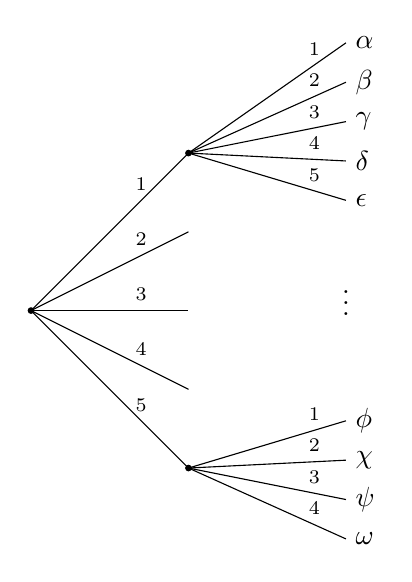
\begin{tikzpicture}[scale=2]
            \filldraw (0, 0) circle (0.5pt);
            \filldraw (1, 1) circle (0.5pt);
            \filldraw (1,-1) circle (0.5pt);
            \foreach \x in {1,...,5}{
                \pgfmathsetmacro\a{(3-\x)/2.0}
                \pgfmathsetmacro\b{(3-\x)/4.0 + 1.2}
                \draw (0, 0) --(1, \a) node[pos=0.7, above] {$\scriptstyle \x$};
                \draw (1, 1) -- (2, \b) node[pos=0.8, above] {$\scriptstyle \x$};
            };
            \foreach \x in {1,...,4}{
                \pgfmathsetmacro\c{(3-\x)/4.0 - 1.2}
                \draw (1, -1) -- (2, \c) node[pos=0.8, above] {$\scriptstyle \x$};
            };
            \node at (2, 0.1) {$\vdots$};
            \node [right] at (2, 1.7) {$\alpha$};
            \node [right] at (2, 1.45) {$\beta$};
            \node [right] at (2, 1.2) {$\gamma$};
            \node [right] at (2, 0.95) {$\delta$};
            \node [right] at (2, 0.7) {$\epsilon$};

            \node [right] at (2, -0.7) {$\phi$};
            \node [right] at (2, -0.95) {$\chi$};
            \node [right] at (2, -1.2) {$\psi$};
            \node [right] at (2, -1.45) {$\omega$};
        \end{tikzpicture}
    \end{center}
    Assuming $f$ is \hyperlink{def:prefixFreeCode}{prefix-free}, no codeword is the ancestor of any other. Now view the tree as a network with water being pumped in at a constant rate and dividing the flow equally at each node.

    The total amount of water we can extract at the codewords is $\sum_{i=1}^m a^{-s_i}$, which is therefore $\leq 1$.

    $(\Leftarrow)$ Conversely, suppose we can construct a prefix-free code with word lengths $s_1, \dotsc, s_m$, wlog $s_1 \leq s_2 \leq \dotsb \leq s_m$.
    We pick codewords of lengths $s_1, s_2, \dotsc$ sequentially ensuring previous codewords are not prefixes.
    Suppose there is no valid choice for the $r$th codeword.
    Then reconstructing the tree as above gives $ \sum_{i=1}^{r-1} a^{-s_i} = 1 $, contradicting our assumption.
    So we can construct a prefix-free code. (There is a more algebraic proof in Welsh.)
\end{proof}

\begin{nthm}[McMillan]\label{thm:mcmillan}
    Every \hyperlink{def:decipherable}{decipherable} \hyperlink{def:code}{code} satisfies \nameref{thm:kraft}.
\end{nthm}

\begin{proof}(Karush)
    Let $f: \Sigma_1 \to \Sigma_2^*$ be a \hyperlink{def:decipherable}{decipherable} \hyperlink{def:code}{code} with word lengths $s_1, \dotsc, s_m$, let $s = \max_{1 \leq i \leq m} s_i$.
    Let $r \in \N$,
    \begin{equation*}
        \left(\sum_{i=1}^m a^{-s_i}\right)^r = \sum_{l=1}^{rs} b_l a^{-l}
    \end{equation*}
    where $b_l$ is the \# of ways of choosing $r$ codewords of total length $l$. $f$ decipherable $\implies b_l \leq \abs{\Sigma_2}^l = a^l$.

    Thus \begin{gather*}\left(\sum_{i=1}^m a^{-s_i}\right)^r \leq \sum_{l=1}^{rs} a^l a^{-l} = rs \\
    \implies \sum_{i=1}^m a^{-s_i} \leq (rs)^{\frac{1}{r}} \to 1 \text{ as } r \to \infty.
    \end{gather*}
    (As $\frac{\log r + \log s}{r} \to 0$ as $r \to \infty$).
    \begin{equation*}
        \therefore \sum_{i=1}^m a^{-s_i} \leq 1.
    \end{equation*}
\end{proof}

\begin{cor}
    A decipherable code with prescribed word lengths exists iff there exists a prefix-free code with the same word lengths.
\end{cor}
So we can restrict our attention to prefix-free codes.

\subsection{Mathematical Entropy}
\begin{defi}[Entropy]\hypertarget{def:entropy}
    The entropy of $X$:
    \begin{equation*}
        H(X) = H(p_1, \dotsc, p_n) = -\sum_{i=1}^n p_i \log p_i
    \end{equation*}
    where, in this course, $\log = \log_2$.
\end{defi}

\begin{remark}
    \leavevmode
    \begin{enumerate}[label=(\roman*)]
        \item If $p_i = 0$, we take $p_i \log p_i=0$.
        \item $\hyperlink{def:entropy}{H(X)} \geq 0$.
    \end{enumerate}
\end{remark}

\begin{eg}
    \leavevmode
    \begin{enumerate}[label=\arabic*.]
        \item Suppose $p_1 = p_2 = p_3 = p_4 = \frac{1}{4}$.
            We identify $\{x_1, x_2, x_3, x_4\}$ with \{HT, HT, TH, TT\}. Then $\hyperlink{def:entropy}{H(X)} = 2$.
        \item Take $(p_1, p_2, p_3, p_4) = (\frac{1}{2}, \frac{1}{4}, \frac{1}{8}, \frac{1}{8})$.
            \begin{center}
                \begin{tikzpicture}[xscale=1.3, yscale=0.8]
                    \draw (0,0) -- (1,1);
                    \draw (0,0) -- (1, -1);
                    \draw (1, -1) -- (2, 0);
                    \draw (1, -1) -- (2, -2);
                    \draw (2, -2) -- (3, -1);
                    \draw (2, -2) -- (3, -3);
                    \node [right] at (1, 1) {$\frac{1}{2}$};
                    \node [right] at (2, 0) {$\frac{1}{4}$};
                    \node [right] at (3, -1) {$\frac{1}{8}$};
                    \node [right] at (3, -3) {$\frac{1}{8}$};
                \end{tikzpicture}
            \end{center}
            \begin{equation*}
                H(X) = \frac{1}{2} \times 1 + \frac{1}{4} \times 2 + \frac{1}{8} \times 3 + \frac{1}{8} \times 3 = \frac{7}{4}.
            \end{equation*}
            So example 1 is more random than example 2.
    \end{enumerate}
\end{eg}

\hyperlink{def:entropy}{Entropy} is a measure of `randomness' or `uncertainty'.
Consider a random variable $X$ taking values $x_1, \dotsc, x_n$ with probability $p_1, \dotsc, p_n$ ($\sum p_i = 1, 0 \leq p_i \leq 1$).
The entropy $H(X)$ is roughly speaking the expected number of tosses of a fair coin needed to simulate $X$ (or the expected number of yes/no questions we need to ask in order to establish the value of $X$).

% Lecture 3
\begin{eg}
    We toss a biased coin, $\Prob(\text{heads}) = p, \Prob(\text{tails}) = 1-p$. Write $H(p) = H(p, 1-p) = -p \log p - (1-p) \log (1-p)$.
    If $p=0$ or $1$, the outcome is certain and so $H(p)=0$. \hyperlink{def:entropy}{Entropy} is maximal where $p=\frac{1}{2}$, i.e. a fair coin.

    \begin{center}
        \begin{tikzpicture}
            \begin{axis}[ axis lines=center, xmin=-0.2, xmax=1.2, ymin=-0.2, ymax=1.2]
            \addplot [domain=0:1, samples=201]
            {-x*log2(x) - (1-x)*log2(1-x)};
            \end{axis}
        \end{tikzpicture}
    \end{center}
\end{eg}

Note the \hyperlink{def:entropy}{entropy} can also be viewed as the expected value of the information of $X$, where information is given by $I(X=x) = -\log_2 \Prob(X=x)$.
For example, if a coin always lands heads we gain no information from tossing the coin.
The entropy is the average amount of information conveyed by a random variable $X$.

\begin{nlemma}[Gibbs' Inequality]\label{lem:gibbs}
    Let $p_1, \dotsc, p_n$ and $q_1, \dotsc, q_n$ be probability distributions. Then
    \begin{equation*}
        -\sum p_i \log p_i \leq -\sum p_i \log q_i
    \end{equation*}
    with equality iff $p_i = q_i$.
\end{nlemma}
\begin{proof}
    Since $\log x = \frac{\ln x}{\ln 2}$ it suffices to prove the inequality with $\log$ replaced with $\ln$.
    Note $\ln x \leq x - 1$, equality iff $x=1$.
    \begin{center}
        \begin{tikzpicture}
            \begin{axis}[axis lines=center, axis equal, xmin=-1, xmax=6]
            \addplot [domain=0:8, samples=201]
            {ln(x)};
            \addplot [domain=-3:8, samples=21]
            {x-1};
            \end{axis}
        \end{tikzpicture}
    \end{center}
    Let $I = \set{1 \leq i \leq n | p_i \neq 0}$
    \begin{align*}
        \ln \frac{q_i}{p_i} &\leq \frac{q_i}{p_i} - 1 \quad \forall i \in I \\
        \sum_{i \in I} p_i \ln \frac{q_i}{p_i} &\leq \sum q_i - \underbrace{\sum p_i}_{=1} \leq 0 \\
        \implies -\sum_{i \in I} p_i \ln p_i &\leq -\sum_{i \in I} p_i \ln q_i \\
        \implies -\sum_{i =1}^n p_i \ln p_i &\leq -\sum_{i =1}^n p_i \ln q_i \\
    \end{align*}
    If equality holds then $\frac{q_i}{p_i} = 1$ $\forall i \in I$. So, $\sum_{i \in I} q_i = 1$ and hence $p_i = q_i$ for $1 \leq i \leq n$.
\end{proof}

\begin{cor}
    $H(p_1, \dotsc, p_n) \leq \log n$ with equality iff $p_1 = p_2 = \dotsb = p_n = \frac{1}{n}$.
\end{cor}
\begin{proof}
    Take $q_1 = q_2 = \dotsc = q_n = \frac{1}{n}$ in \nameref{lem:gibbs}.
\end{proof}

Suppose we have two alphabets $\Sigma_1, \Sigma_2$ with $\abs{\Sigma_1} = m$ and $\abs{\Sigma_2} = a$, for $m \geq 2$ and $a \geq 2$.
We model the source as a sequence of random variables $X_1, X_2, \dotsc$ taking values in $\Sigma_1$.
\begin{defi}[Memoryless source]\hypertarget{def:memoryless}
    A \textbf{Bernoulli} or \textbf{memoryless} source is a sequence of independently, identically distributed random variables.
\end{defi}
That is, for each $\mu \in \Sigma_1$, $\Prob(X_i = \mu)$ is independent of $i$ and independent of all past and future symbols emitted. Thus
\begin{equation*}
    \Prob(X_1= x_1, X_2 = x_2, \dotsc, X_k = x_k) = \prod_{i = 1}^k \Prob(X_i = x_i).
\end{equation*}
Let $\Sigma_1 = \{\mu_1, \dotsc, \mu_n\}$, $p_i = \Prob(X=\mu_i)$ (assume $p_i > 0$).
\begin{defi}[Expected word length]\hypertarget{def:ewl}
    The \textbf{expected word length} of a code $f: \Sigma_1 \to \Sigma_2^*$ with word lengths $s_1, \dotsc, s_m$ is $E(S) = \sum_{i=1}^m p_i s_i$.
\end{defi}

\begin{defi}[Optimal code]\hypertarget{def:optCode}
    A \hyperlink{def:code}{code} $f:\Sigma_1 \to \Sigma_2^*$ is \textbf{optimal} if it has the shortest possible \hyperlink{def:ewl}{expected word length} among \hyperlink{def:decipherable}{decipherable} codes.
\end{defi}
\begin{nthm}[Shannon's Noiseless Coding Theorem]\label{thm:noiselessCode}
    The minimum \hyperlink{def:ewl}{expected word length} of a \hyperlink{def:decipherable}{decipherable code} $f: \Sigma_1 \to \Sigma_2^*$ satisfies
    \begin{equation*}
        \frac{H(X)}{\log a} \leq E(S) < \frac{H(X)}{\log a} + 1
    \end{equation*}
\end{nthm}
\begin{proof}
    The lower bound is given by combining \nameref{lem:gibbs} and \nameref{thm:kraft}.
    Let $q_i = \frac{a^{-s_i}}{c}$ where $c = \sum a^{-s_i} \leq 1$ by \nameref*{thm:kraft}.
    Note $\sum q_i = 1$.
    \begin{align*}
        H(X) = -\sum p_i \log p_i &\leq -\sum_i p_i \log q_i \\
                                  &= \sum p_i (s_i \log a + \log c) \\
                                  &= \left(\sum p_i s_i\right) \log a + \underbrace{\log c}_{\leq 0} \leq E(S) \log a\\
        \implies \frac{H(X)}{\log a} &\leq E(S)
    \end{align*}
    We get equality $\iff p_i = a^{-s_i}$ for some integers $s_i$.
    For the upper bound put
    \begin{equation*}
        s_i = \ceil{-\log_a p_i}
    \end{equation*}
    where $\ceil{x}$ means least integer $\geq x$.

    We have
    \begin{gather*}
        - \log_a p_i \leq s_i < - \log_a p_i + 1 \\
        \implies a^{-s_i} \leq p_i \implies \sum a^{-s_i} \leq \sum p_i \leq 1.
    \end{gather*}
    So by \cref{thm:kraft}, $\exists$ a prefix-free code with word lengths $s_1, \dotsc, s_m$.
    Also,
    \begin{align*}
        E(S) &= \sum p_i s_i \\
             &< p_i (- \log_a p_i + 1) \\
             &= \frac{H(X)}{\log a} + 1 \qedhere
    \end{align*}
\end{proof}
\begin{remark}
    The lower bound holds for all \hyperlink{def:decipherable}{decipherable} \hyperlink{def:code}{codes}.
\end{remark}

\subsection{Shannon-Fano coding}
Follows from above proof.
\hypertarget{def:shannonFanoCode}Set $s_i = \ceil{-\log_a p_i}$ and construct a \hyperlink{def:prefixFreeCode}{prefix-free code} with word lengths $s_1, \dotsc, s_m$ by taking the $s_i$ in increasing order ensuring that previous \hyperlink{def:code}{codewords} are not prefixes.
\nameref{thm:kraft} ensures there is enough room.
\begin{eg}
    Suppose $\mu_1, \dotsc, \mu_5$ are emitted with probabilities $0.4, 0.2, 0.2, 0.1, 0.1$.

    A \hypertarget{ex:shannonfano1}{possible \hyperlink{def:shannonFanoCode}{Shannon-Fano}} code (with $a=2$, $\Sigma_2 = \{0, 1\}$) has
    \begin{center}
    \begin{tabular}{c c c}
        $p_i$ & $\ceil{-\log_2 p_i}$ & \\
        \hline
        0.4 & 2 & 00 \\
        0.2 & 3 & 010 \\
        0.2 & 3 & 100 \\
        0.1 & 4 & 1100 \\
        0.1 & 4 & 1110
    \end{tabular}
    \end{center}
    This has \hyperlink{def:ewl}{expected word length}
    \begin{align*}
        &= 2 \times 0.4 + 3 \times 0.2 + 3 \times 0.2 + 4 \times 0.1 + 4 \times 0.1 \\
        &= 2.8.
    \end{align*}
    compare $H(X) \approx 2.12$.
\end{eg}

% Lecture 4
\subsection{Huffman coding}
For simplicity, take $a=2$.
Take $\Sigma_1=\{\mu_1, \dotsc, \mu_m\}$ with $p_i = \Prob(X = \mu_i)$. Without loss of generality, $p_1 \geq p_2 \geq \dotsb \geq p_m$.
\hypertarget{def:huffmanCode}Huffman coding is defined inductively.

If $m=2$, assign codewords $0$ and $1$. If $\mu > 2$, find a Huffman coding in the case of messages $\mu_1, \mu_2, \dotsc, \nu$, with probabilities $p_1, p_2, \dotsc, p_{m-1} + p_m$.

Append $0$ (resp, $1$) to the codeword for $\nu$ to give a codeword for $\mu_{m-1}$ (resp, $\mu_m$).

\begin{remark}
    \leavevmode
    \begin{enumerate}[label=\roman*)]
        \item This construction gives a \hyperlink{def:prefixFreeCode}{prefix-free} code.
        \item We exercise some choice when some of the $p_i$ are equal. So \hyperlink{def:huffmanCode}{Huffman codes} are not unique.
    \end{enumerate}
\end{remark}

\begin{eg}
    Use the same \hyperlink{ex:shannonfano1}{example probabilities} as earlier.
    \begin{equation*}
        \begin{tikzcd}[column sep=large, arrows={start anchor=east, end anchor=west, dash}]
                0.4 \quad \color{bblue}(1)
              & 0.4 \quad \color{bblue}(1)
              & 0.4 \quad \color{bblue}(1)
              & 0.6 \quad \color{bblue}({\color{bred}0}) \\
                0.2 \quad \color{bblue}(00)
              & 0.2 \quad \color{bblue}(00)
              & 0.4 \quad \color{bblue}(0{\color{bred}1}) \ar[ur]
              & 0.4 \quad \color{bblue}(1) \\
                0.2 \quad \color{bblue}(011)
              & 0.2 \quad \color{bblue}(01{\color{bred}1}) \ar[ur]
              & 0.2 \quad \color{bblue}(0{\color{bred}0}) \ar[uur] \\
                0.1 \quad \color{bblue}(010{\color{bred}1}) \ar[r]
              & 0.2 \quad \color{bblue}(01{\color{bred}0}) \ar[uur] \\
                0.1 \quad \color{bblue}(010{\color{bred}0}) \ar[ur]
    \end{tikzcd}
    \end{equation*}
    So $\{1, 00, 011, 0101, 0100\}$ is the \hyperlink{def:prefixFreeCode}{prefix-free code} constructed. The \hyperlink{def:ewl}{expected word length} is:
    \begin{align*}
        &= 1 \times 0.4 + 2 \times 0.2 + 2 \times 0.2 + 4 \times 0.1 + 4 \times 0.1 \\
        &= 0.4 + 0.4 + 0.6 + 0.4 + 0.4\\
        &= 2.2.
    \end{align*}
    This is better than \hyperlink{def:shannonFanoCode}{Shannon-Fano}, which gave 2.8.
\end{eg}

\begin{nthm}\label{thm:huffOpt}
    \hyperlink{def:huffmanCode}{Huffman coding} is \hyperlink{def:optCode}{optimal}.
\end{nthm}
\begin{nlemma}\label{lem:1.6}
    Suppose we have $\mu_1, \dotsc, \mu_m \in \Sigma_1$ emitted with probabilities $p_1, \dotsc, p_m$.
    Let $f$ be an \hyperlink{def:optCode}{optimal} \hyperlink{def:prefixFreeCode}{prefix-free} \hyperlink{def:code}{code}, with word lengths $s_1, \dotsc, s_m$.
    Then
    \begin{enumerate}[label=\roman*)]
        \item If $p_i > p_j$, then $s_i \leq s_j$.
        \item $\exists$ two \hyperlink{def:code}{codewords} of maximal length which are equal up to the last digit.
    \end{enumerate}
\end{nlemma}

\begin{proof}
    \leavevmode
    \begin{enumerate}[label=\roman*)]
        \item If not, then swap the $i$th and $j$th \hyperlink{def:codewords}{codewords}.
            This decreases the \hyperlink{def:ewl}{expected word length}, contradicting $f$ \hyperlink{def:optCode}{optimal}.
        \item If not, then either only one codeword of maximal length, or any two codewords of maximal length differ before the last digit.
            In either case, delete the last digit of each codeword of maximal length.
            This maintains the \hyperlink{def:prefixFreeCode}{prefix-free} condition, contradicting $f$ optimal. \qedhere
    \end{enumerate}
\end{proof}
\begin{proof}[Proof of \cref{thm:huffOpt}]
    We only take the case $a=2$.
    We show by induction on $m$ that any \hyperlink{def:huffmanCode}{Huffman code} of size $m$ is \hyperlink{def:optCode}{optimal}. \\
    For $m=2$, \hyperlink{def:code}{codewords} $0,1$ are optimal. \\
    For $m>2$, say source $X_m$ emits $\mu_1, \dotsc, \mu_m$ with probabilities $p_1 \geq p_2 \geq \dotsc \geq p_m$ while source $X_{m-1}$ emits $\mu_1, \dotsc, \mu_{m-2}, \nu$ with probabilities $p_1, \dotsc, p_{m-2}, p_{m-1} + p_m$.

    We construct a Huffman coding $f_{m-1}$ for $X_{m-1}$ and extend to a Huffman coding for $X_m$.
    Then the \hyperlink{def:ewl}{expected codeword length} satisfies:
    \begin{equation*}
        E(s_m) = E(s_{m-1}) + p_{m-1} + p_m \label{eq:4dag} \tag{$\dagger$}
    \end{equation*}
    Let $f_m'$ be an optimal code for $X_m$, WLOG $f_m'$ prefix-free.
    \Cref{lem:1.6} tells us that by shuffling codewords, we may assume that the last two codewords are of maximal length and differ only in the last digit, say $y_0$ and $y_1$ for some string $y$.

    We define a code $f_{m-1}'$ for $X_{m-1}$ with
    \begin{align*}
        f_{m-1}'(\mu_i) &= f'_m(\mu_i) \quad \forall 1 \leq i \leq m-2 \\
        f'_{m-1}(\nu) &= y.
    \end{align*}
    Then $f'_{m-1}$ is a prefix-free code, and the expected word length satisfies
    \begin{equation*}
        E(s'_m) = E(s'_{m-1}) + p_{m-1} + p_m \tag{$\ddagger$} \label{eq:4ddag}
    \end{equation*}
    Induction hypothesis tells us $f_{m-1}$ is optimal, so $E(s_{m-1}) \leq E(s'_{m-1})$. Hence $E(s_m) \leq E(s'_m)$ by \eqref{eq:4dag}, \eqref{eq:4ddag}.
    So $f_m$ optimal.
\end{proof}
\begin{remark}
    Not all \hyperlink{def:optCode}{optimal} codes are \hyperlink{def:huffmanCode}{Huffman}. For instance, take $m=4$, and probabilities $0.3, 0.3, 0.2, 0.2$. An optimal code is given by $00, 01, 10, 11$, but this is not Huffman.

    But, the previous result says that if we have a prefix-free optimal code with word lengths $s_1, \dotsc, s_m$ and associated probabilites $p_1, \dotsc, p_m$, $\exists$ a Huffman code with these word lengths.
\end{remark}

\begin{defi}[Joint entropy]\hypertarget{def:jointEntropy}
    The \textbf{joint entropy} of $X$ and $Y$ is
    \begin{equation*}
        H(X,Y) = - \sum_{x \in \Sigma_1} \sum_{y \in \Sigma_2} \Prob(X=x, Y=y) \log \Prob(X=x, Y=y).
    \end{equation*}
\end{defi}

\begin{nlemma}\label{lem:1.7}
    $\hyperlink{def:jointEntropy}{H(X, Y)} \leq \hyperlink{def:entropy}{H}(X) + H(Y)$, with equality $\iff X,Y$ independent.
\end{nlemma}

\begin{proof}
    Take $\Sigma_1 = \{x_1, \dotsc, x_m\}$, $\Sigma_2 = \{y_1, \dotsc, y_n\}$. Let $p_{ij} = \Prob(X=x_i, Y=y_j)$, as well as $p_i = \Prob(X=x_i)$, $q_i = \Prob(Y=y_i)$.
    Apply \nameref{lem:gibbs} to the distributions $p_{ij}$ and $p_i q_j$:
    \begin{align*}
        -\sum p_{ij} \log(p_{ij}) &\leq -\sum p_{ij} \log(p_i q_j) \\
                                  &= - \sum_i \left(\sum_j p_{ij} \log p_i\right) - \sum_j \left(\sum_i p_{ij} \log q_j\right) \\
                                  &= -\sum p_i \log p_i - \sum q_j \log q_j
    \end{align*}
    That is, $H(X,Y) \leq H(X) + H(Y)$.
    Equality $\iff p_{ij} = p_i q_j \forall i, j \iff X, Y$ independent.
\end{proof}

% Lecture 5
Suppose a source $\Omega$ produces a stream $X_1, X_2, \dotsc$ of random variables with values in $\Sigma$.
The probability mass function (p.m.f.) of $X^{(n)} = (X_1, \dotsc, X_n)$ is given by
\begin{equation*}p_n(x_1, \dotsc, x_n) = \Prob(X_1, \dotsc, X_n = x_1, \dotsc, x_n) \quad \forall x_1, \dotsc, x_n \in \Sigma^n\end{equation*}
Now,
\begin{align*}
    p_n &: \Sigma^n \to \R \\
    X^{(n)} &: \Omega \to \Sigma^n\\
    \shortintertext{can form}
    p_n(X^{(n)})&: \Sigma \xrightarrow{X^{(n)}} \Sigma^n \xrightarrow{p_n} \R
\end{align*}
a random variable sending $\omega \mapsto p_n(X^{(n)} = X^{(n)} (\omega))$.
\begin{eg}
    Take $\Sigma = \{A, B, C\}$, with
    \begin{equation*}
        X^{(2)} =
        \begin{cases}
            AB & p=0.3 \\
            AC & p=0.1 \\
            BC & p=0.1 \\
            BA & p=0.2 \\
            CA & p=0.25 \\
            CB & p=0.05 \\
        \end{cases}
    \end{equation*}
    So, $p_2(AB) = 0.3$, etc, and $p_2(X^{(2)})$ takes values
    \begin{equation*}
        p_2(X^{(2)}) =
        \begin{cases}
            0.3 & p=0.3 \\
            0.1 & p=0.2 \\
            0.2 & p=0.2 \\
            0.25 & p=0.25 \\
            0.05 & p=0.05 \\
        \end{cases}
    \end{equation*}
\end{eg}

\begin{defi}[Convergence in probability]\hypertarget{def:probConverge}
    A sequence of random variables $X_1, X_2, \dotsc$ \textbf{converges in probability} to $c \in \R$, written $X_n \xlongrightarrow{p} c$ as $n \to \infty$, if
    \begin{equation*}
        \forall \epsilon > 0 \quad \Prob(\abs{X_n - c} \leq \epsilon) \to 1 \quad \text{as } n \to \infty.
    \end{equation*}
    So, $X_n$ and $c$ can take very different values for large $n$, but only on a set with small probability.
\end{defi}

\begin{thm}[Weak law of large numbers]\hypertarget{def:wlln}
    $X_1, X_2, \dotsc$ an independent, identically distributed sequence of random variables with finite expected value $\mu$, then
    \begin{equation*}
        \frac{1}{n} \sum_{i=1}^n X_i \probConv \mu \quad \text{as } n \to \infty.
    \end{equation*}
\end{thm}
\begin{eg}[Application]
    Take $X_1, X_2, \dotsc$ a \hyperlink{def:memoryless}{Bernoulli source}. Then $p(X_1), p(X_2), \dotsc$ are i.i.d. random variables
    \begin{align*}
        p(X_1, \dotsc, X_n) &= p(X_1) \dotsc p(X_n) \\
        -\frac{1}{n} \log p(X_1, \dotsc, X_n) &= -\frac{1}{n} \sum_{i=1}^n \log p(X_i) \probConv E(-\log p(X_1)) = H(X_1) \quad \text{as } n \to \infty.
    \end{align*}
\end{eg}
\begin{defi}[Asymptotic Equipartition Property]
    \leavevmode

    A source $X_1, X_2, \dotsc$ satisfies the \hypertarget{def:aep}{\textbf{Asymptotic Equipartition Property}} (AEP) if for some $H\geq 0$ we have
    \begin{equation*}
        -\frac{1}{n} \log p(X_1, \dotsc, X_n) \xrightarrow{p} H \quad \text{as } n \to \infty.
    \end{equation*}
\end{defi}
\begin{eg}
    Consider a coin, $p(H) = p$. If coin tossed $N$ times, expect approximately $pN$ heads and $(1-p)N$ tails.
    \begin{align*}
        &\Prob(\text{particular sequence of $pN$ heads and $(1-p)N$ tails}) \\
        =&p^{pN} (1-p)^{(1-p)N}\\
        =&2^{N(p \log p) + (1-p) \log (1-p)} = 2^{-N H(A)}
    \end{align*}
    where $A$ is the result of an independent coin toss.
    So, with high probability we will get a typical sequence, and its probability will be close to $2^{-NH(A)}$.
\end{eg}
\begin{nlemma}\label{lem:1.8}
    A source $X_1, \dotsc, X_n$ satisfies \hyperlink{def:aep}{AEP} iff it satisfies the following.
    \begin{gather*}
        \forall \epsilon > 0, \, \exists n_0(\epsilon) \text{ such that } \forall n \geq n_0(\epsilon) \, \exists \text{ a `\hypertarget{def:typicalSet}{typical set}' } T_n \subset \Sigma^n \text{ with}
    \end{gather*}
    \begin{equation*}
        \begin{gathered}
        \Prob((X_1, \dotsc, X_n) \in T_n) > 1 - \epsilon \\
        2^{-n(H+\epsilon)} \leq p(x_1, \dotsc, x_n) \leq 2^{-n(H-\epsilon)}\quad \forall (x_1, \dotsc, x_n) \in T^n
        \end{gathered}
        \tag{$*$} \label{eq:5star}
    \end{equation*}
\end{nlemma}
\begin{proof}[Sketch proof]
    \hyperlink{def:aep}{AEP} $\Rightarrow$ \eqref{eq:5star}.
    Take
    \begin{align*}
        T_n &= \Set{(x_1, \dotsc, x_n) \in \Sigma^n | \abs{-\frac{1}{n} \log p(x_1, \dotsc, x_n) - H} < \epsilon} \\
            &= \Set{(x_1, \dotsc, x_n) \in \Sigma^n | 2^{-n(H+\epsilon)} \leq p(x_1, \dotsc, x_n) \leq 2^{-n(H-\epsilon)}} \\
    \end{align*}
    \eqref{eq:5star} $\Rightarrow$ \hyperlink{def:aep}{AEP}
    \begin{equation*}
        \Prob\left(\abs{- \frac{1}{n} p(X_1, \dotsc, X_n) - H} < \epsilon\right) \geq \Prob(T_n) \to 1 \quad \text{as } n \to \infty. \qedhere
    \end{equation*}
\end{proof}
\begin{defi}[Reliably encodable]\hypertarget{def:reliablyEncode}
    A source $X_1, X_2, \dotsc$ is \textbf{reliably encodable} at rate $r$ if $\exists A_n \subset \Sigma^n$ for each $n$ such that
    \begin{enumerate}[label=(\roman*)]
        \item $\frac{\log \abs{A_n}}{n} \to r \quad \text{as } n \to \infty$
        \item $\Prob((X_1, \dotsc, X_n) \in A_n) \to 1 \quad \text{as } n \to \infty$.
    \end{enumerate}
    So, in principle you can encode at rate almost $r$ with negligible error for long enough strings.
\end{defi}
So, if $\abs{\Sigma}=a$, you can \hyperlink{def:reliablyEncode}{reliably encode} at rate $\log a$. However you can often do better.
For example, consider telegraph English with 26 letters and a space. $27 \approx 2^{4.756}$, so can encode at rate of $4.76$ bits/letter. But much lower rates suffice, as there is a lot of redundancy in the English language.
Hence the following definition.
\begin{defi}[Information rate]\hypertarget{def:informationRate}
    The \textbf{information rate} $H$ of a source is the infimum of all values at which it is \hyperlink{def:reliablyEncode}{reliably encodable}.
\end{defi}
Roughly, $nH$ is the number of bits required to encode $(X_1, \dotsc, X_n)$.
\begin{nthm}[Shannon's first coding theorem]
    If a source satisfies \hyperlink{def:aep}{AEP} with some constant $H$, then the source has information rate $H$.
\end{nthm}
\begin{proof}Let $\epsilon > 0$ and let $T_n \subset \Sigma^n$ be \hyperlink{def:typicalSet}{typical sets}.
    Then for sufficiently large $n \geq n_0(\epsilon)$,
    \begin{equation*}
        p(x_1, \dotsc, x_n) \geq 2^{-n (H + \epsilon))} \quad \forall (x_1, \dotsc, x_n) \in T^n.
    \end{equation*}
    So,
    \begin{gather*}
        \Prob(\left(X_1, \dotsc, X_n\right) \in T_n) \geq 2^{-n(H+\epsilon)} \abs{T_n} \\
        \implies \abs{T_n} \leq 2^{n(H+\epsilon)}
    \end{gather*}
    therefore the source is \hyperlink{def:reliablyEncode}{reliably encodable} at rate $H+\epsilon$.

    Conversely, if $H=0$, done. Otherwise, pick $0 < \epsilon < \frac{H}{2}$. Suppose the source is reliably encodable at rate $H - 2 \epsilon$, say with sets $A_n$.
    \begin{gather*}
        p(x_1, \dotsc, x_n) \leq 2^{-n(H-\epsilon)} \quad \forall (x_1, \dotsc, x_n) \in T_n \\
        \begin{aligned}
            \implies \Prob((x_1, \dotsc, x_n) \in A_n \cap T_n) &\leq 2^{-n (H-\epsilon)} \abs{A_n} \\
            \implies \frac{\log \Prob(A_n \cap T_n)}{n} &\leq -(H-\epsilon) + \frac{\log \abs{A_n}}{n} \\
                                                    &\to -(H-\epsilon) + (H-2 \epsilon) = -\epsilon \quad \text{as } n \to \infty \\
            \implies \log \Prob(A^n \cap T_n) &\to -\infty \\
            \implies \Prob(A_n \cap T_n) &\to 0
        \end{aligned}
    \end{gather*}
    But $\Prob(T_n) \to 1$ as $n \to \infty$ and $\Prob(A_n) \to 1$ as $n \to \infty$, a contradiction.
    So, the source is not reliably encodable at rate $H-2\epsilon$, and so the information rate is $H$.
\end{proof}

% Lecture 6
\clearpage
\section{Error Control Codes}
\begin{defi}[Binary code]\hypertarget{def:binaryCode}
    A $[n, m]$ \textbf{binary code} is a subset $C \subset \{0, 1\}^n$ of size $\abs{C}=m$. We say $C$ has length $n$.
    The elements of $C$ are called \textbf{codewords}.
\end{defi}
We use a $[n, m]$-code to send one of $m$ possible messages through a \hyperlink{def:bsc}{BSC} making use of the channel $n$ times.
\begin{center}
    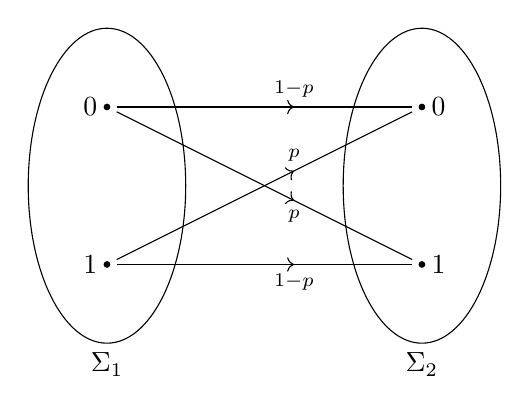
\begin{tikzpicture}
        \draw (-2, 0) circle [x radius=1cm, y radius=2cm] node [below=2cm] {$\Sigma_1$};
        \draw ( 2, 0) circle [x radius=1cm, y radius=2cm] node [below=2cm] {$\Sigma_2$};

        \node (0l) at (-2, 1) {};
        \node (1l) at (-2,-1) {};

        \node (0r) at (2, 1) {};
        \node (1r) at (2,-1) {};

        \filldraw (0l) circle (1pt) node [left] {0};
        \filldraw (1l) circle (1pt) node [left] {1};
        \filldraw (0r) circle (1pt) node [right] {0};
        \filldraw (1r) circle (1pt) node [right] {1};

        \begin{scope}[decoration={
            markings,
            mark=at position 0.6 with {\arrow{>}}}
            ]
            \draw[postaction={decorate}] (0l) -- (0r)
                node [above,align=center,pos=0.6] {$\scriptstyle 1-p$};
            \draw[postaction={decorate}] (0l) -- (1r)
                node [below,align=center,pos=0.6] {$\scriptstyle p$};
            \draw[postaction={decorate}] (1l) -- (0r)
                node [above,align=center,pos=0.6] {$\scriptstyle p$};
            \draw[postaction={decorate}] (1l) -- (1r)
                node [below,align=center,pos=0.6] {$\scriptstyle 1-p$};
        \end{scope}
    \end{tikzpicture}
\end{center}
\begin{defi}[Information rate]\hypertarget{def:infoRate}
    The \textbf{information rate} of $C$ is
    \begin{equation*}
        \rho(C) = \frac{\log{m}}{n}
    \end{equation*}
    where we continue to use $\log = \log_2$.
\end{defi}

Note since $C\subset\{0, 1\}^n$, $\rho(C) \leq 1$, with equality iff $C = \{0, 1\}^n$.
A \hyperlink{def:binaryCode}{code} with size $m=1$ has \hyperlink{def:infoRate}{information rate} 0.

We aim to design codes with both a large information rate and a small error rate, which are contradicting aims.
The error rate depends on the decoding rule. We consider 3 possible rules.
\begin{enumerate}[label=(\roman*)]\hypertarget{def:idealObserver}
    \item The \textbf{ideal observer} decoding rule decodes $x \in \{0, 1\}^n$ as the \hyperlink{def:binaryCode}{codeword} $c$ maximising $\Prob(c\text{ sent} \mid x\text{ received})$.
    \item \hypertarget{def:maximumLikelihood}{The} \textbf{maximum likelihood} decoding rule decodes $x \in \{0, 1\}^n$ as the codeword $c$ maximising $\Prob(x\text{ received} \mid c\text{ sent})$.
    \item \hypertarget{def:minimumDistanceRule}{The} \textbf{minimum distance} decoding rule decodes $x \in \{0, 1\}^n$ as the codeword $c$ minimising $\#\set{1 \leq i \leq n | x_i \neq c_i}$.
\end{enumerate}
\begin{remark}
    Some convention should be agreed in the case of a `tie', e.g.\ choose at random, or ask for message to be sent again.
\end{remark}
\begin{nlemma}\label{lem:2.1}
    If all messages are equally likely, then the \hyperlink{def:idealObserver}{ideal observer} and \hyperlink{def:maximumLikelihood}{maximum likelihood rule} agree.
\end{nlemma}
\begin{proof}
    By Bayes' rule,
    \begin{align*}
        \Prob(c \text{ sent} \mid x \text{ received}) &= \frac{\Prob(c \text{ sent}, x \text{ received})}{\Prob(x \text{ received})} \\
                                               &= \frac{\Prob(c \text{ sent})}{\Prob(x \text{ received})} \Prob(x \text{ received} \mid c \text{ sent}).
    \end{align*}
    We suppose $\Prob(c \text{ sent})$ is independent of $c$. So for fixed $x$, maximising $\Prob(c \text{ sent} \mid x \text{ received}) $ is the same as maximising $\Prob(x \text{ received} \mid c \text{ sent})$.
\end{proof}

\begin{defi}[Hamming distance]\label{def:hammingDistance}
    Let $x, y \in \{0, 1\}^n$. Then \textbf{Hamming distance} between $x$ and $y$ is
    \begin{equation*}d(x, y) = \# \set{1 \leq i \leq n | x_i \neq y_i}.\end{equation*}
\end{defi}
\begin{nlemma}\label{lem:2.2}
    If $p < \frac{1}{2}$, then \hyperlink{def:maximumLikelihood}{maximum likelihood} and \hyperlink{def:minimumDistanceRule}{minimum distance} agree.
\end{nlemma}
\begin{proof}
    Suppose $\hyperlink{def:hammingDistance}{d(x, c)} = r$,
    \begin{equation*}
        \Prob(x \text{ received} \mid c \text{ sent}) = p^r (1-p)^{n-r} = (1-p)^n \left(\frac{p}{1-p}\right)^r.
    \end{equation*}
    Since $p < \frac{1}{2}$, $\frac{p}{1-p} < 1$. So choosing $c$ to maximise $\Prob(x \text{ received} \mid c \text{ sent})$ is the same as choosing $c$ to minimise $d(x, c)$.
\end{proof}
Note we assumed $p < \frac{1}{2}$, which is not unreasonable.
\begin{eg}
    Suppose codewords $000$ and $111$ are sent with probabilities $\alpha = \frac{9}{10}$ and $1-\alpha = \frac{1}{10}$ respectively. We use a \hyperlink{def:bsc}{BSC} with $p = \frac{1}{4}$.
    If we receive $110$, how should it be decoded?
    Clearly \hyperlink{def:minimumDistanceRule}{minimum distance} and therefore \hyperlink{def:maximumLikelihood}{maximum likelihood} (by \cref{lem:2.2}) say decode as $111$.
    For \hyperlink{def:idealObserver}{ideal observer:}
    \begin{align*}
        \Prob(000 \text{ sent} \mid 110 \text{ received}) &= \frac{\Prob(000 \text{ sent} , 110 \text{ received})}{\Prob(110 \text{ received})} \\
                                                   &= \frac{\alpha p^2 (1-p)}{\alpha p^2 (1-p) + (1-\alpha) p (1-p)^2} \\
                                                   &= \frac{\alpha p}{\alpha p + (1-\alpha) (1-p)} \\
                                                   &= \frac{9/40}{9/40 + 3/40} = \frac{3}{4} \\
        \Prob(111 \text{ sent} \mid 110 \text{ received}) &= \frac{(1-\alpha) p^2 (1-p)}{(1-\alpha) p^2 (1-p) + \alpha p (1-p)^2} \\
                                                   &= \frac{(1-\alpha)(1-p)}{(1-\alpha)(1-p) + \alpha p} \\
                                                   &= \frac{3/40}{9/40 + 3/40} = \frac{1}{4}.
    \end{align*}
    So the ideal observer rule says decode as $000$.
\end{eg}
\begin{remark}
    The \hyperlink{def:idealObserver}{ideal observer} rule is also known as the minimum-error rule.
    But it does rely on knowing the probabilities of the codewords sent.
\end{remark}
From now on, we use \hyperlink{def:minimumDistanceRule}{minimum distance} decoding.
\begin{defi}
    For a \hyperlink{def:binaryCode}{binary code} $C$,
    \begin{enumerate}[label=(\roman*)]
        \item $C$ is \hypertarget{def:errorDet}{\textbf{$d$-error detecting}} if changing at most $d$ letters of a codeword cannot give another codeword.
        \item $C$ is \hypertarget{def:errorCor}{\textbf{$e$-error correcting}} if knowing that the string received has at most $e$ errors is sufficient to determine which codeword was sent.
    \end{enumerate}
\end{defi}
\begin{eg} \leavevmode
    \begin{enumerate}[label=\arabic*.]
        \item The \hypertarget{def:repetitionCode}{repetition code} of length $n$ has:
            \begin{equation*}
                C = \{\underbrace{0\dotsm0}_n, \underbrace{1 \dotsm1}_n\}
            \end{equation*}
            This is an \hyperlink{def:binaryCode}{$[n, 2]$-code}. It is $n-1$ \hyperlink{def:errorDet}{error detecting}, and $\floor{\frac{n-1}{2}}$ \hyperlink{def:errorCor}{error correcting}.
            But it has \hyperlink{def:infoRate}{information rate} $= \frac{1}{n}$.
        \item The \hypertarget{def:parityCheckCode}{simple parity check} code of length $n$ (also known as paper tape code).
            We view $\{0, 1\} = \mathbb{F}_2 = \Z/2\Z$ (i.e.\ do arithmetic modulo $2$).
            \begin{equation*}
                C = \Set{(x_1, \dotsc, x_n) \in \{0, 1\}^n | \sum_{i=1}^n x_i = 0}.
            \end{equation*}
            This is a \hyperlink{def:binaryCode}{$[n, 2^{n-1}]$-code}.
            It is $1$-\hyperlink{def:errorDet}{error detecting} and $0$-\hyperlink{def:errorCor}{error correcting}.
            It has \hyperlink{def:infoRate}{information rate} $\frac{n-1}{n}$.
        \item \hypertarget{def:hammingCode}{Hamming's original} code (1950). % this example was lecture 7
            Let $C \subseteq \mathbb{F}_2^7$ be defined by
            \begin{align*}
                c_1 + c_3 + c_5 + c_7 &= 0 \\
                c_2 + c_3 + c_6 + c_7 &= 0 \\
                c_4 + c_5 + c_6 + c_7 &= 0
            \end{align*}
            where all arithmetic is modulo 2.
            Since we may choose $c_3, c_5, c_6, c_7$ freely, the $c_1, c_2, c_4$ are uniquely determined.
            So we get $\abs{C} = 2^4$ i.e.\ $C$ is a $[7,16]$-\hyperlink{def:binaryCode}{code}.
            It has \hyperlink{def:infoRate}{information rate} $\frac{\log m} {n} = \frac{4}{7}$.
            Note $c_{3,5,6,7}$ are free, $c_{1,2,4}$ are check digits.

            Suppose we receive $x \in \mathbb{F}_2^7$. We form the syndrome $z_x = (z_1, z_2, z_4)$ where
            \begin{align*}
                z_1 &= x_1 + x_3 + x_5 + x_7 \\
                z_2 &= x_2 + x_3 + x_6 + x_7 \\
                z_4 &= x_4 + x_5 + x_6 + x_7.
            \end{align*}
            If $x \in C$, then $z = (0,0,0)$. If $\hyperlink{def:hammingDistance}{d}(x, c) = 1$ for some $c \in C$, then the place where $x$ and $c$ differ is given by $z_1 + 2 z_2 + 4z_4$ (not modulo 2).
            Since if $x = c+ e_i$ where $e_i = 0\dotso 010\dotso 0$ ($1$ in the $i$th place), then the syndrome of $x$ is the syndrome of $e_i$.
            For example the syndrome of $e_3$ is $(1, 1, 0)$, the binary expansion of $3$.
            True in fact for each $1 \leq i \leq 7$.
    \end{enumerate}
\end{eg}

\begin{remark}
    Suppose we change our \hyperlink{def:binaryCode}{code} $C \subset \{0, 1\}^n$ by using the same permutation to reorder each \hyperlink{def:binaryCode}{codeword}.
    This gives a code with the same mathematical properties (e.g.\ \hyperlink{def:infoRate}{information rate}, \hyperlink{def:errorDet}{error detection rate}).
    We say such codes are equivalent.
\end{remark}

% Lecture 7

\begin{nlemma}\label{lem:2.3}
    The \hyperlink{def:hammingDistance}{Hamming distance} is a metric on $\mathbb{F}_2^n$.
\end{nlemma}

\begin{proof}
    Clearly $d(x, y) \geq 0$ with equality iff $x=y$.
    Also $d(x, y) = d(y, x)$. Check triangle inequality, let $x, y, z \in \mathbb{F}_2^n$:
    \begin{gather*}
        \set{1 \leq i \leq n | x_i \neq z_i} \subseteq
        \set{1 \leq i \leq n | x_i \neq y_i} \cup
        \set{1 \leq i \leq n | y_i \neq z_i} \\
        \implies d(x, z) \leq d(x, y) + d(y, z) \qedhere
    \end{gather*}
\end{proof}
\begin{remark}
    We could also write $d(x, y) = \sum_{i=1}^n d_1(x_i, y_i)$ where $d_1$ is the discrete metric on $\{0, 1\}$.
\end{remark}

\begin{defi}[Minimum distance]\label{def:minimumDistanceCode}
    The \textbf{minimum distance} of a code $C$ is the smallest \hyperlink{def:hammingDistance}{Hamming distance} between distinct codewords.
\end{defi}
\begin{notation}
    An \hyperlink{def:binaryCode}{$[n, m]$-code} with \hyperlink{def:minimumDistanceCode}{minimum distance} $d$ is sometimes called an \hypertarget{def:nmdCode}{$\bm{[n, m, d]}$\textbf{-code}}.
\end{notation}
\begin{remark}\leavevmode
    \begin{itemize}
        \item $m \leq 2^n$, with equality if $C = \mathbb{F}_2^n$, this is called the \hypertarget{def:trivialCode}{trivial code}.
        \item $d \leq n$, with equality in the case of the \hyperlink{def:repetitionCode}{repetition code}.
    \end{itemize}
\end{remark}
\begin{nlemma}\label{lem:2.4}
    Let $C$ be a \hyperlink{def:binaryCode}{code} with \hyperlink{def:minimumDistanceCode}{minimum distance} $d$.
    \begin{enumerate}[label=(\roman*)]
        \item $C$ is $(d-1)$-\hyperlink{def:errorDet}{error detecting}, but cannot detect all sets of errors.
        \item $C$ is $\floor{\frac{d-1}{2}}$-\hyperlink{def:errorCor}{error correcting}, but cannot correct all sets of $\floor{\frac{d-1}{2}} + 1$ errors.
    \end{enumerate}
\end{nlemma}
\begin{proof}\leavevmode
    \begin{enumerate}[label=(\roman*)]
        \item If $x \in \mathbb{F}_2^n$ and $c \in C$ with $1 \leq d(x, c) \leq d-1$ then $x \notin C$. So errors are detected.
            Suppose $c_1, c_2 \in C$ with $\hyperlink{def:hammingDistance}{d(c_1, c_2)} = d$.
            Then $c_1$ can be corrupted to $c_2$ with just $d$ errors, this set of errors will not be detected.
        \item Let $e = \floor{\frac{d-1}{2}}$, so $e \leq \floor{\frac{d-1}{2}} < e+1$, i.e.\ $2e < d \leq 2(e+1)$.
            Let $x \in \mathbb{F}_2^n$. If $\exists c_1 \in C$ with $d(x, c_1) \leq e$, we want to show $d(x, c_2) > e \quad \forall c_2 \in C, c_2 \neq c_1$.
            By the triangle inequality,
            \begin{align*}
                d(x, c_2) &\geq d(c_1, c_2) - d(x, c_1) \\
                          &\geq d - e \\
                          &> e
            \end{align*}
            so $C$ is $e$-error correcting.

            Let $c_1, c_2 \in C$ with $d(c_1, c_2) = d$. Let $x \in \mathbb{F}_2^n$ differ from $c_1$ in precisely $e+1$ places, where $c_1$ and $c_2$ differ.
            Then $d(x, c_1) = e+1$ and $d(x, c_2) = d - (e+1) \leq e+1$.
            So $C$ cannot correct all $e+1$ errors.
    \end{enumerate}
\end{proof}
\begin{eg}
    \leavevmode
    \begin{enumerate}[label=\arabic*)]
        \item The \hyperlink{def:repetitionCode}{repetition code} is a \hyperlink{def:nmdCode}{$[n, 2, n]$-code}, it is $n-1$ \hyperlink{def:errorDet}{error detecting} and $\floor{\frac{n-1}{2}}$ \hyperlink{def:errorCor}{error correcting}.
        \item The simple \hyperlink{def:parityCheckCode}{parity check} code is a $[n, 2^{n-1}, 2]$-code, it is $1$-error detecting and $0$-error correcting.
        \item \hyperlink{def:hammingCode}{Hamming's original} $[7, 16]$-code is $1$-error correcting $\implies d \geq 3$. Since 0000000 and 1110000 are both valid \hyperlink{def:binaryCode}{codewords}, $d=3$. That is, it is a $[7, 16, 3]$-code.
    \end{enumerate}
\end{eg}

\subsection{New codes from old}
Let $C$ be an \hyperlink{def:nmdCode}{$[n,m,d]$-code}.
\begin{enumerate}[label=\roman*)]
    \item The \hypertarget{def:parityExtension}{parity extension} of $C$ is
        \begin{equation*}
            \overline{C} = \Set{(c_1, c_2, \dotsc, c_n, \sum c_i) | (c_1, \dotsc, c_n) \in C}.
        \end{equation*}
        It is a $[n+1, m, d']$ code, for $d' = d$ or $d+1$, depending on $d$ being odd or even.
    \item Fix $1 \leq i \leq n$. Deleting the $i$th letter from each codeword gives a \hypertarget{def:puncturedCode}{punctured code}.  If $d \geq 2$, the new code is $[n-1, m, d'']$ for $d'' = d-1$ or $d$.
    \item Fix $1 \leq i \leq n$ and $a \in \{0, 1\}$. The shortened code is
        \begin{equation*}
            \set{(c_1, \dotsc, c_{i-1}, c_{i+1}, \dotsc, c_n) | (c_1, \dotsc, c_{i-1}, a, c_{i+1}, \dotsc, c_n) \in C}.
        \end{equation*}
        It is a $[n-1, m', d']$-code, where $d' \geq d$ and some choice of $a$ gives $m' \geq \frac{m}{2}$.
\end{enumerate}

% Lecture 8
\subsection{Bound on codes}
\begin{defi}[Hamming ball]
    Let $x \in \mathbb{F}_2^n$ and $r \geq 0$. The (closed) \hypertarget{def:hammingBall}{\textbf{Hamming ball}} with centre $x$ and radius $r$ is
    \begin{equation*}
        B(x, r) = \set{y \in \mathbb{F}_2^n | \hyperlink{def:hammingDistance}{d}(x, y) \leq r}.
    \end{equation*}
    Note the `volume'
    \begin{equation*}
        V(n, r) = \abs{B(x, r)} = \sum_{i=0}^r \binom{n}{i}
    \end{equation*}
    which is independent of $x$.
\end{defi}
\begin{nlemma}[Hamming's bound]\label{lem:2.5}
    If $C \subset \mathbb{F}_2^n$ is $e$-\hyperlink{def:errorCor}{error correcting}, then
    \begin{equation*}
        \abs{C} \leq \frac{2^n}{V(n, e)}.
    \end{equation*}
\end{nlemma}
\begin{proof}
    Since $C$ is $e$-\hyperlink{def:errorCor}{error correcting}, the \hyperlink{def:hammingBall}{Hamming balls} $B(c, e)$ are disjoint for $c \in C$.
    So
    \begin{align*}
        \sum_{c \in C} \abs{B(c, e)} &\leq \abs{\mathbb{F}_2^n} \\
        \implies \abs{C} V(n, e) &\leq 2^n \\
        \implies \abs{C} &\leq \frac{2^n}{V(n, e)}.\qedhere
    \end{align*}
\end{proof}
\begin{defi}[Perfect code]
    A \hyperlink{def:binaryCode}{$[n, m]$-code} which can \hyperlink{def:errorCor}{correct} $e$ errors is called \textbf{\hypertarget{def:perfect}perfect} if \begin{equation*}m = \frac{2^n}{V(n, e)}.\end{equation*}
\end{defi}

\begin{remark}
    If $\frac{2^n}{V(n, e)} \notin \Z$, then no perfect $e$-\hyperlink{def:errorCor}{error correcting} code of length $n$ can exist.
\end{remark}
\begin{eg}
    \hyperlink{def:hammingCode}{Hamming's original $[7,16,3]$-code}, can \hyperlink{def:errorCor}{correct} $1$ error.
    \begin{equation*}
        \frac{2^n}{V(n, e)} = \frac{2^7}{V(7, 1)} = \frac{2^7}{1 + 7} = 2^4 = m
    \end{equation*}
    so it is a \hyperlink{def:perfect}{perfect code}.
\end{eg}
\begin{remark}
    A \hyperlink{def:perfect}{perfect} $e$-\hyperlink{def:errorCor}{error correcting} code will always incorrectly decode $e+1$ errors.
\end{remark}
\begin{defi}[Maximum size of code\hypertarget{def:bestCode}]
    \begin{equation*}
        A(n, d) = \max\set{m | \exists \text{ a } [n, m, d]\text{-code}}
    \end{equation*}
    i.e.\ size of largest code with parameters $n$ and $d$ .
\end{defi}
\begin{eg}
    $\hyperlink{def:bestCode}{A(n, 1)} = 2^n$, the \hyperlink{def:trivialCode}{trivial code} = $\mathbb{F}_2^n$. $A(n, n) = 2$, for the \hyperlink{def:repetitionCode}{repetition code}.
\end{eg}
\begin{nprop}[Gilbert-Shannon-Varshanov bound]\label{prop:2.6}
    \begin{equation*}
        \frac{2^n}{V(n, d-1)} \underset{\mathclap{
            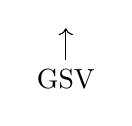
\begin{tikzpicture}
                \node[below] (A) at (0, 0) {GSV};
                \draw[->] (A) to (0, 0.4);
            \end{tikzpicture}
        }}{\leq} A(n, d)
        \underset{\mathclap{
            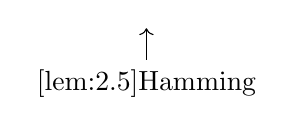
\begin{tikzpicture}
                \node[below] (A) at (0, 0) {\hyperref[lem:2.5]{Hamming}};
                \draw[->] (A) to (0, 0.4);
            \end{tikzpicture}
        }}{\leq}
        \frac{2^n}{V(n, \floor{\frac{d-1}{2}})}
    \end{equation*}
\end{nprop}
\begin{proof}
    Let $C$ be a code of length $n$ and \hyperlink{def:minimumDistanceCode}{minimum distance} $d$ of largest possible size.
    Then $\nexists x \in \mathbb{F}_2^n$ such that $d(x, c) \geq d \quad \forall c \in C$, otherwise we would replace $C$ with $C \cup \{x\}$
    \begin{align*}
        \implies \mathbb{F}_2^n &\subseteq \bigcup_{c \in C}B(c, d-1) \\
        \implies 2^n &\leq \abs{C} V(n, d-1) \\
        \implies \abs{C} &\geq \frac{2^n}{V(n, d-1)}. \qedhere
    \end{align*}
\end{proof}
\begin{eg}
    Take $n=10$, $d=3$.
    \begin{align*}
        V(n, 1) &= 1 + 10 = 11 \\
        V(n, 2) &= 1 + 10 + \binom{10}{2} = 56
    \end{align*}
    \Cref{prop:2.6} gives $\frac{2^{10}}{56} \leq A(10, 3) \leq \frac{2^{10}}{11}$, so $19 \leq A(10, 3) \leq 93$. The exact value $A(10, 3) = 72$ was only found in 1999.
\end{eg}
There exist asymptotic versions of the \nameref{prop:2.6} and \nameref{lem:2.5}.
Let
\begin{equation*}\alpha(\delta) = \limsup \frac{1}{n} \log A(n, \delta n), \quad 0 \leq \delta \leq 1.\end{equation*}
\begin{notation}
    $H(\delta) = -\delta \log \delta - (1-\delta) \log (1-\delta)$.
\end{notation}
The asymptotic GSV says
\begin{equation*}
    \alpha(\delta) \geq 1 - H(\delta) \quad \text{for } 0 <\delta < \frac{1}{2}
\end{equation*}
while the asymptotic Hamming bound says
\begin{equation*}
    \alpha(\delta) \leq 1 - H\left(\frac{\delta}{2}\right).
\end{equation*}
We prove the asymptotic GSV bound
\begin{nprop}\label{prop:2.7}
    Let $0 < \delta < \frac{1}{2}$. Then
    \begin{enumerate}[label=(\roman*)]
        \item $\log V(n, \floor{n \delta}) \leq n H(\delta)$
        \item $\frac{\log A(n, \floor{n \delta})}{n} \geq 1 - H(\delta)$
    \end{enumerate}
\end{nprop}
\begin{proof}[Proof (i) $\Rightarrow$ (ii)]
    The \nameref{prop:2.6} gives
    \begin{align*}
        A(n, \floor{n \delta}) &\geq \frac{2^n}{V(n, \floor{n \delta} - 1)} \\
                               &\geq \frac{2^n}{V(n, \floor{n \delta})} \\
        \implies \log A(n, \floor{n \delta}) &\geq n - \log V(n, \floor{n \delta})\\
                                             &\geq n - n H(\delta) \qquad \text{by (i)} \\
        \implies \frac{\log A(n, \floor{n\delta})}{n} &\geq 1 - H(\delta) \qedhere
    \end{align*}
\end{proof}
\begin{proof}[Proof of (i)]
    \begin{align*}
        1 = (\delta + (1-\delta))^n &= \sum_{i=0}^n \binom{n}{i}\delta^i (1-\delta)^{n-i} \\
                                    &\geq \sum_{i=0}^{\floor{n \delta}} \binom{n}{i} \delta^i (1 - \delta)^{n-i} \\
                                    &= (1-\delta)^n \sum_{i=0}^{\floor{n\delta}} \binom{n}{i} \left(\frac{\delta}{1 - \delta}\right)^i\\
                                    &\geq (1-\delta)^n \sum_{i = 0}^{\floor{n \delta}} \binom{n}{i} \left(\frac{\delta}{1-\delta}\right)^{n\delta}\\
        1&\geq \delta^{n \delta} (1-\delta)^{n(1-\delta)} V(n, \floor{n\delta}) \\
        \implies 0 &\geq n(\delta \log \delta + (1-\delta) \log (1-\delta)) + \log V(n, \floor{n \delta}) \\
        \implies \log V(n, \floor{n \delta}) &\leq n H(\delta). \qedhere
    \end{align*}
\end{proof}
\subsection{Channel Capacity}
Let $\abs{\Sigma} = q$. A code of length $n$ is a subset of $\Sigma^n$ (usually we take $q=2$).

A code is used to send messages through a \hyperlink{def:dmc}{discrete memoryless channel} with $q$ input letters.
For each code a decoding rule is chosen.

\begin{defi}[Maximum error probability]\hypertarget{def:ehat}
    The \textbf{maximum error probability} is
    \begin{equation*}
        \hat{e}(C) = \max_{c \in C} \Prob(\text{error} \mid c \text{ sent}).
    \end{equation*}
\end{defi}
\begin{defi}[Reliable transmission]\hypertarget{def:relTrans}
    A channel can transmit \textbf{reliably at rate $R$} if there exists a sequence of codes $C_1, C_2, \dotsc$ where $C_n$ is a code of length $n$ and size $\floor{2^{nR}}$ such that
    \begin{equation*}
        \hyperlink{def:ehat}{\hat{e}(C_n)} \to 0 \text{ as } n \to \infty.
    \end{equation*}
\end{defi}
\begin{defi}\hypertarget{def:capacity}
    The (operational) \textbf{channel capacity} is the supremum over all \hyperlink{def:relTrans}{reliable transmission} rates.
\end{defi}

% Lecture 9
\begin{nlemma}\label{lem:2.8}
    Let $\epsilon > 0$. A \hyperlink{def:bsc}{BSC} with error probability $p$ is used to send $n$ digits. Then
    \begin{equation*}
        \Prob(\text{BSC makes} \geq n(p + \epsilon) \text{ errors}) \to 0 \text{ as } n \to \infty.
    \end{equation*}
\end{nlemma}
\begin{proof}
    Let
    \begin{equation*}
        \mu_i =
        \begin{cases*}
            1 & if digit mistransmitted \\
            0 & otherwise
        \end{cases*}
    \end{equation*}
    $\mu_1, \mu_2, \mu_3, \dotsc$ are i.i.d.\ random variables.
    \begin{align*}
        \begin{rcases}
            \Prob(\mu_i = 1) = p \\
            \Prob(\mu_i = 0) = 1-p
        \end{rcases}
        \implies \Exp(\mu_i) &= p \\
        \Prob(\text{BSC makes} \geq n(p + \epsilon) \text{ errors}) &= \Prob\left(\sum_{i=1}^n \mu_i \geq n(p + \epsilon)\right) \\
                                                                    &\leq \Prob\left(\abs{\frac{1}{n} \sum \mu_i - p} \geq \epsilon\right)
    \end{align*}
    This $\to 0$ as $n \to \infty$ by \hyperlink{def:wlln}{WLLN}.
\end{proof}
\begin{remark}
    $\sum_{i=1}^n \mu_i$ is a binomial random variable with parameters $n$ and $p$.
\end{remark}
\begin{nprop}\label{prop:2.9}
    The \hyperlink{def:capacity}{capacity} of a \hyperlink{def:bsc}{BSC} with error probability $p<\frac{1}{4}$ is $\neq 0$.
\end{nprop}
\begin{proof}
    Choose $\delta$ with $2 p < \delta < \frac{1}{2}$. We prove \hyperlink{def:relTrans}{reliably encoding} at rate $R = 1 - H(\delta) > 0$.
    Let $C_n$ be the largest code of length $n$ and \hyperlink{def:minimumDistanceCode}{minimum distance} $\floor n \delta$.
    \begin{align*}
        \abs{C_n} = A(n, \floor{n \delta}) &\geq 2^{n (1 - H(\delta))} \qquad \text{by \cref{prop:2.7}}
                                           &= 2^{nR}.
    \end{align*}
    Replacing $C_n$ by a subcode gives $\abs{C_n} = \floor{2^{nR}}$ and still minimum distance $\geq \floor{n\delta}$.
    Using \hyperlink{def:minimumDistanceRule}{minimum distance decoding},
    \begin{align}
        \hyperlink{def:ehat}{\hat{e}(C_n)} &\leq \Prob(\text{\hyperlink{def:bsc}{BSC} makes} \geq \floor{\frac{\floor{n \delta}-1}{2}} \text{errors}) \\
        &\leq \Prob(\text{\hyperlink{def:bsc}{BSC} makes} \geq \floor{\frac{n \delta-1}{2}} \text{errors}). \\
    \end{align}
    Pick $\epsilon > 0$ such that $p + \epsilon < \frac{\delta}{2}$.
    Then $\frac{n \delta - 1}{2} = n \left(\frac{\delta}{2} - \frac{1}{2n}\right) > n(p+\epsilon)$ for $n$ sufficiently large.
    Therefore, $\hat{e}(C_n) \leq \Prob(\text{BSC makes} \geq n(p+\epsilon) \text{errors}) \to 0$ as $ n \to \infty$ by \cref{lem:2.8}.
\end{proof}

\subsection{Conditional Entropy}
\begin{defi}[Conditional Entropy]\hypertarget{def:condH}
    Let $X$ and $Y$ be random variables taking values in $\Sigma_1$ and $\Sigma_2$. We define
    \begin{align*}
        H(X \mid Y = y) &= -\sum_{x \in \Sigma_1} \Prob(X = x \mid Y=y) \log \Prob(X=x \mid Y=y) \\
        H(X \mid Y) &= \sum_{y \in \Sigma_2} \Prob(Y = y) H(X \mid Y=y).
    \end{align*}
\end{defi}
\begin{nlemma}\label{lem:2.10}
$\hyperlink{def:jointEntropy}{H(X, Y)} = \hyperlink{def:condH}{H(X \mid Y)} + \hyperlink{def:entropy}{H(Y)}$
\end{nlemma}
\begin{proof}
    \begin{align*}
        H(X \mid Y) &= -\sum_{y \in \Sigma_2} \sum_{x \in \Sigma_1} \Prob(X = x \mid Y = y) \Prob(Y = y) \log \Prob(X = x \mid Y = y) \\
                 &= -\sum_{y \in \Sigma_2} \sum_{x \in \Sigma_1} \Prob(X = x , Y = y) \log \left(\frac{\Prob(X = x , Y = y)}{\Prob(Y = y)}\right) \\
            & \begin{multlined} =-\sum_{y \in \Sigma_2} \sum_{x \in \Sigma_1} \Prob(X=x,Y=y) \log \Prob(X=x,Y=y)\\ + \sum_{y\in \Sigma_2} \left(\sum_{x \in \Sigma_1} \Prob(X=x,Y=y)\right) \log \Prob(Y=y)
        \end{multlined} \\
                 &= H(X, Y) - H(Y). \qedhere
    \end{align*}
\end{proof}

\begin{eg}
    A fair six-sided dice is thrown. $X$ is the value on the dice,
    \begin{align*}
        Y &=
        \begin{dcases*}
            0 & if $X$ even\\
            1 & if $X$ odd\\
        \end{dcases*}
        \\
        H(X, Y) &= H(X) = \log 6 \qquad H(Y) = \log 2 = 1 \\
        H(X \mid Y) &= H(X, Y) - H(Y) = \log 3 \\
        H(Y, X) &= 0.
    \end{align*}
\end{eg}
\begin{cor}
    $\hyperlink{def:condH}{H(X\mid Y)} \leq \hyperlink{def:entropy}{H(X)}$ with equality iff $X$ and $Y$ are independent.
\end{cor}

\begin{proof}
    Since $H(X \mid Y) = \hyperlink{def:jointEntropy}{H(X, Y)} - H(Y)$, this is equivalent to showing $H(X, Y) \leq H(X) + H(Y)$ with equality iff $X$ and $Y$ are independent. We showed this in \cref{lem:1.7}.
\end{proof}

\begin{notation}
    In the definition of conditional entropy we can replace random variables $X$ and $Y$ with random vectors $\vec{X} = (X_1, \dotsc, X_r)$ and $\vec{Y} = (Y_1,  \dotsc, Y_s)$.  This defines
    \begin{equation*}H(X_1, \dotsc, X_r \mid Y_1, \dotsc, Y_s) \coloneqq H(\vec{X}, \vec{Y}).\end{equation*}
\end{notation}

\begin{nlemma}\label{lem:2.11}
    $\hyperlink{def:condH}{H(X \mid Y)} \leq H(X \mid Y , Z) + \hyperlink{def:entropy}{H(Z)}.$
\end{nlemma}

\begin{proof}
    We expand $H(X, Y, Z)$ using \cref{lem:2.10} in two different ways.
    \begin{align*}
        H(X, Y, Z) &= H(Z \mid X, Y) + H(X \mid Y) + H(Y) \\
        H(X, Y, Z) &= H(X \mid Y, Z) + H(Z \mid Y) + H(Y) \\
        \shortintertext{Since $H(Z\mid X,Y) \geq 0$,}
        H(X \mid Y) &\leq H(X \mid Y, Z) + H(Z \mid Y) \leq H(X \mid Y, Z) + H(Z). \qedhere
    \end{align*}
\end{proof}

\begin{nlemma}[Fano's inequality]\label{lem:2.12}
    Let $X,Y$ be random variables taking values in $\Sigma_1$ with $\abs{\Sigma_1} = m$.
    Let $p  = P(X \neq Y)$. Then $\hyperlink{def:condH}{H(X \mid Y)} \leq H(p) + p \log(m-1)$.
\end{nlemma}

\begin{proof}
    Let
    \begin{equation*}
        Z =
        \begin{dcases}
            1 & \text{if } X \neq Y \\
            0 & \text{if } X = Y \\
        \end{dcases}
    \end{equation*}
    so $P(Z=1)=p$ and $P(Z=0) = 1-p$.
    By \cref{lem:2.11},
    \begin{equation*}H(X \mid Y) \leq H(X \mid Y, Z) + H(Z) = H(X \mid Y, Z) + H(p).\end{equation*}
    Now,
    \begin{align*}
        &H(X \mid Y = y, Z=0)=0, &&\text{as $Z=0$ implies $X = Y$}\\
        &H(X \mid Y = y, Z=1) \leq \log(m-1) &&\text{since $m-1$ choices for $X$ remain.}
    \end{align*}
    So,
    \begin{align*}
        H(X \mid Y, Z) &= \sum_{y, z} \Prob(Y=y, Z=z) H(X \mid Y=y, Z=z) \\
                    &\leq \sum_y \Prob(Y=y, Z=1) \log(m-1)  \\
                    &= \Prob(Z=1) \log(m-1). \qedhere
    \end{align*}
\end{proof}

% Lecture 10
\begin{defi}[Mutual information]\hypertarget{def:mutInfo}
    Let $X, Y$ be random variables. The \textbf{mutual information} is $ I(X; Y) = \hyperlink{def:entropy}{H(X)} - \hyperlink{def:condH}{H(X \mid Y)} $ i.e.\ the amount of information about $X$ conveyed by $Y$.
\end{defi}

By \cref{lem:1.7} and \cref{lem:2.10}, $\hyperlink{def:mutInfo}{I(X;Y)} = \hyperlink{def:entropy}{H(X)} + H(Y) - \hyperlink{def:jointEntropy}{H(X,Y)} \geq 0$ with equality iff $X$ and $Y$ are independent.
Note the symmetry $I(X;Y) = I(Y;X)$.

Consider a \hyperlink{def:dmc}{DMC}. Let $X$ take values in $\Sigma_1$, where $\abs{\Sigma_1} = m$ with probabilities $p_1, \dotsc, p_m$.
Let $Y$ be the random variables output when the channel is given input $X$.

\begin{defi}[Information channel capacity]\hypertarget{def:infoChannelCapacity}
    \leavevmode
    The \textbf{information channel capacity} is \begin{equation*}\max_X \hyperlink{def:mutInfo}{I(X;Y)}.\end{equation*}
\end{defi}

\begin{remark}\leavevmode
    \begin{enumerate}[label=(\roman*)]
        \item The maximum is over all choices of $p_1, \dotsc, p_m$.
        \item The maximum is attained, since we have a continuous function on the compact set $\set{(p_1, \dotsc, p_m) | p_i \geq 0, \sum p_i = 1} \subset \R^n$.
        \item The information capacity only depends on the channel matrix.
    \end{enumerate}
\end{remark}

\begin{nthm}[Shannon's Second Coding Theorem]\label{thm:2.13}
    \hyperlink{def:capacity}{Operational capacity} = \hyperlink{def:infoChannelCapacity}{information capacity}.
\end{nthm}
We will show $\leq$ in general, $\geq$ for a \hyperlink{def:bsc}{BSC}.
We now compute the capacity of certain channels using \cref{thm:2.13}.

\subsubsection*{Capacity of a \hyperlink{def:bsc}{Binary Symmetric Channel}}
Take error probability $p$.

\begin{center}
    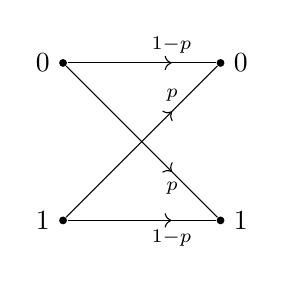
\begin{tikzpicture}
        \begin{scope}[every node/.append style={circle,fill=black,inner sep=1pt}]
            \node [label=left:{0}] (0l) at (-1, 1) {};
            \node [label=left:{1}] (1l) at (-1,-1) {};

            \node [label=right:{0}] (0r) at (1, 1) {};
            \node [label=right:{1}] (1r) at (1,-1) {};
        \end{scope}

        \begin{scope}[decoration={markings, mark=at position 0.7 with {\arrow{>}}}, every node/.append style={align=center,pos=0.7}]
            \draw[postaction={decorate}] (0l) -- (0r) node [above] {$\scriptstyle 1-p$};
            \draw[postaction={decorate}] (0l) -- (1r) node [below] {$\scriptstyle p$};
            \draw[postaction={decorate}] (1l) -- (0r) node [above] {$\scriptstyle p$};
            \draw[postaction={decorate}] (1l) -- (1r) node [below] {$\scriptstyle 1-p$};
        \end{scope}
    \end{tikzpicture}
\end{center}
\begin{align*}
    \text{Input $X$:} \qquad \Prob(X=0) &= 1-\alpha \\
    \Prob(X=1) &= \alpha \\
    \text{Output $Y$:} \qquad
    \Prob(Y=0) &= (1-\alpha)(1-p) + \alpha p \\
    \Prob(Y=1) &= \alpha (1-p) + (1-\alpha) p
\end{align*}
\begin{align*}
    \text{\hyperlink{def:infoChannelCapacity}{Capacity is } }C &= \max_\alpha \hyperlink{def:mutInfo}{I(X;Y)} \\
      &= \max_\alpha (\hyperlink{def:entropy}{H(Y)} - \hyperlink{def:condH}{H(Y \mid X)}) \\
      &= \max_\alpha (H(\alpha(1-p) + (1-\alpha) p) - H(p)) \\
    \intertext{since $H(Y \mid X) = \Prob(X=0)H(p) + \Prob(X=1)H(p) = H(p)$}
    &= 1 - H(p) \\
    &= 1 + p \log p + (1-p) \log(1-p)
\end{align*}

\begin{center}
    \begin{tikzpicture}
        \begin{axis}[ axis lines=center, xmin=-0.2, xmax=1.2, ymin=-0.2, ymax=1.2]
        \addplot [domain=0:1, samples=201]
        {1+x*log2(x) + (1-x)*log2(1-x)};
        \end{axis}
    \end{tikzpicture}
\end{center}

\subsubsection*{Capacity of Binary Erasure Channel}
Again, take error probability $p$.
\begin{center}
    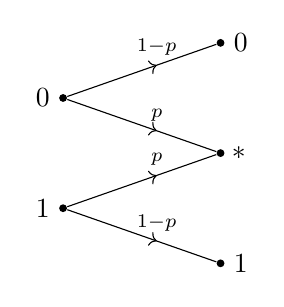
\begin{tikzpicture}[yscale=0.7]
        \begin{scope}[every node/.style={circle,fill=black,inner sep=1pt}]
            \node [label=left:0] (0l) at (-1, 1) {};
            \node [label=left:1] (1l) at (-1,-1) {};

            \node [label=right:0] (0r) at (1, 2) {};
            \node [label=right:$*$] (*r) at (1, 0) {};
            \node [label=right:1] (1r) at (1,-2) {};
        \end{scope}
        \begin{scope}[decoration={ markings, mark=at position 0.6 with {\arrow{>}}}, every node/.style={align=center,pos=0.6,above}]
            \draw[postaction={decorate}] (0l) -- (0r) node {$\scriptstyle 1-p$};
            \draw[postaction={decorate}] (0l) -- (*r) node {$\scriptstyle p$};
            \draw[postaction={decorate}] (1l) -- (*r) node {$\scriptstyle p$};
            \draw[postaction={decorate}] (1l) -- (1r) node {$\scriptstyle 1-p$};
        \end{scope}
    \end{tikzpicture}
\end{center}
\begin{align*}
    \text{Input $X$:} \qquad \Prob(X=0) &= 1-\alpha \\
    \Prob(X=1) &= \alpha \\
    \text{Output $Y$:} \qquad
    \Prob(Y=0) &= (1-\alpha)(1-p)\\
    \Prob(Y=1) &= \alpha (1-p) \\
    \Prob(Y=*) &= p
\end{align*}
We have $H(X \mid Y=0) = 0$, $H(X \mid Y=1)=0$.
\begin{gather*}
    H(X \mid Y=*) = - \sum_x \Prob(X=x \mid Y=*) \log \Prob(X=x \mid Y=*) \\
    \Prob(X=0 \mid Y=*) = \frac{\Prob(X=0, Y=*)}{\Prob(Y=*)} = \frac{(1-\alpha)p}{p} = 1-\alpha.
\end{gather*}
Similarly, $\Prob(X=1 \mid Y=*) = \alpha$.
So $H(X \mid Y=*) = H(\alpha)$, so $H(X \mid Y) = p H(\alpha)$.

\begin{align*}
    \text{\hyperlink{def:infoChannelCapacity}{Capacity is } }C &= \max_\alpha \hyperlink{def:mutInfo}{I(X;Y)} \\
      &= \max_\alpha (\hyperlink{def:entropy}{H(X)} - \hyperlink{def:condH}{H(X \mid Y)}) \\
      &= \max_\alpha (H(\alpha) - pH(\alpha)) \\
      &= (1-p) \max_\alpha H(\alpha) \\
      &= 1 -p, \quad \text{attained when } \alpha = \tfrac{1}{2}.
\end{align*}

We model using a channel $n$ times as the $n$th extension, i.e.\ replace input and output alphabets $\Sigma_1$ and $\Sigma_2$ by $\Sigma_1^n$ and $\Sigma_2^n$ with channel probabilities
\begin{equation*}
    \Prob(y_1, \dotsc, y_n \text{ received} \mid x_1, \dotsc, x_n \text{ sent}) = \prod_{i=1}^n \Prob(y_i \text{ received} \mid x_i \text{ sent})
\end{equation*}

\begin{nlemma}\label{lem:2.14}
    The $n$th extension of a \hyperlink{def:dmc}{DMC} with information capacity $C$ has information capacity $nC$.
\end{nlemma}
\begin{proof}
    We take random variable input $(X_1, \dotsc, X_n) = \vec{X}$ producing random variable output $(Y_1, \dotsc, Y_n) = \vec{Y}$.
    Now, $\hyperlink{def:condH}{H(\vec{Y} \mid \vec{X})} = \sum_{\vec{x}} \Prob(\vec{X} = \vec{x}) H(\vec{Y} \mid \vec{X}=\vec{x})$.
    Since the channel is memoryless, $H(\vec{Y} \mid \vec{X} = \vec{x}) = \sum_i H(Y_i \mid \vec{X} = \vec{x}) = \sum_i H(Y_i \mid X_i = x_i)$.
    So,
    \begin{align*}
        H(\vec{Y} \mid \vec{X}) &= \sum_{\vec{x}} \Prob(\vec{X}=\vec{x}) \sum_i H(Y_i \mid X_i = x_i) \\
                             &= \sum_i \sum_n H(Y_i \mid X_i = u) \Prob(X_i = u) \\
                             &= \sum_i H(Y_i \mid X_i).
    \end{align*}
    Now $H(\vec{Y}) \leq \hyperlink{def:entropy}{H(Y_1)} + \dotsb + H(Y_n)$ by \cref{lem:1.7}, thus
    \begin{align*}
        \hyperlink{def:mutInfo}{I(X; Y)} &= H(\vec{Y}) - H(\vec{Y} \mid \vec{X}) \\
                                         &\leq \sum_i (H(Y_i) - H(Y_i \mid X_i)) \\
                                         &= \sum_i I(X_i ; Y_i) \\
                                         &\leq nC \quad \text{by definition of \hyperlink{def:infoChannelCapacity}{information capacity}}.
    \end{align*}
    For equality, need $Y_1, \dotsc, Y_n$ to be independent. This can be achieved by taking $X_1, \dotsc, X_n$ independent and choosing the distribution such that $I(X_i; Y_i) = c$.
\end{proof}

% Lecture 11
\begin{nprop}\label{prop:2.15}
    For a \hyperlink{def:dmc}{DMC}, \hyperlink{def:capacity}{operational capacity} $\leq$ \hyperlink{def:infoChannelCapacity}{information capacity}.
\end{nprop}
\begin{proof}
    Let $C$ be the \hyperlink{def:infoChannelCapacity}{information capacity}.
    Suppose we can \hyperlink{def:relTrans}{transmit reliably} at rate $R > C$, i.e.\ there is a sequence of codes $(C_n)_{n \geq 1}$ with $C_n$ of length $n$ and size $\floor{2^{nR}}$ such that $\hyperlink{def:ehat}{\hat{e}}(C_n) \to 0$ as $n \to \infty$.
    \begin{align*}
        \text{Recall } \hat{e}(C_n) &= \max_{c \in C_n} \Prob(\text{error} \mid c \text{ sent}). \\
        \hypertarget{def:e}{\text{Let } e(C_n)} &= \frac{1}{\abs{C_n}} \sum_{c \in C_n} \Prob(\text{error} \mid c \text{ sent}).
    \end{align*}
    Clearly $e(C_n) \leq \hat{e}(C_n)$, so $e(C_n) \to 0$ as $n \to \infty$.
    Take random variable input $X$, equidistributed over $C_n$.
    Let $Y$ be the random variable output when $X$ is transmitted and decoded.
    So $e(C_n) = P(X \neq Y) = p$, say.
    \begin{align*}
        H(X) &= \log \abs{C_n} \geq n R - 1 \text{ for large } n. \\
        H(X \mid Y) &\leq H(p) + p \log(\abs{C_n} - 1) \text{ by \nameref{lem:2.12}} \\
                    &\leq 1 + pnR \\
        I(X;Y)&= H(X) - H(X \mid Y) \\
        n C &\geq n R - 1 - (1 + p n R) \\
        \implies p n R &\geq n(R-C) - 2 \\
        \implies p &\geq \frac{n(R-C) - 2}{nR} \nrightarrow 0 \text{ as } n \to \infty.
    \end{align*}
    Thus our sequence of codes cannot exist.
\end{proof}

\begin{nprop}\label{prop:2.16}
    Consider a \hyperlink{def:bsc}{BSC}, error probability $p$.
    Let $R < 1 - \hyperlink{def:entropy}{H(p)}$.
    Then $\exists$ a sequence of codes $(C_n)_{n \geq 1}$ of length $n$ and size $\floor{2^{nR}}$ such that $\hyperlink{def:e}{e(C_n)} \to 0$ as $n \to \infty$.
\end{nprop}
\begin{proof}
    Idea: Construct codes by picking codewords at random.
    Without loss of generality $p < \frac{1}{2}$, so $\exists \epsilon > 0$ such that $R < 1 - H(p+\epsilon)$.
    We use \hyperlink{def:minimumDistanceRule}{minimum distance decoding} (in case of tie, make arbitrary choice).
    Let $m = \floor{2^{nR}}$.
    We pick a \hyperlink{def:binaryCode}{$[n, m]$-code} $C$ at random (i.e.\ each word with probability).
    Say $C = \{c_1, \dotsc, c_m\}$.

    Choose $1 \leq i \leq m$ at random (i.e.\ each with probability $\frac{1}{m}$).
    We send $c_i$ through the channel and get output $Y$.
    Then $\Prob(Y \text{ is not decoded as } c_i)$ is the average value of $e(C)$ as $C$ runs over all $[n,m]$-codes.
    We can pick $C_n$ a $[n, m]$-code with $e(C_n)$ at most this average.
    So it will suffice to show
    $\Prob(Y \text{ is not decoded as } c_i) \to 0$ as $n \to \infty$.

    Let $r = \floor{n (p+\epsilon)}$.
    \begin{equation*}\Prob(Y \text{ is not decoded as } c_i) \leq \Prob(c_i \notin B(y, r)) + \Prob(B(Y, r) \cap C \supsetneq \{c_i\}).\end{equation*}
    We now split into two cases: (i) $d(c_i, Y) > r$ or (ii) $d(c_i, Y) \leq r$.
    \begin{enumerate}[label=(\roman*)]
        \item \begin{equation*}\begin{aligned}[t]
                \Prob(d(c_i, Y) > r) &= \Prob(\text{BSC makes} >r \text{ errors}) \\
                                     &= \Prob(\text{BSC makes} >n(p+\epsilon) \text{ errors}) \\
                                     &\to 0 \text{ as } n \to \infty \text{ by \cref{lem:2.8}}.
            \end{aligned}\end{equation*}
        \item If $j \neq i$,
            \begin{align*}
                \Prob(c_j \in B(Y, r) \mid c_i \in B(Y, r)) &= \frac{V(n, r) - 1}{2^n - 1} \leq \frac{V(n, r)}{2^n} \\
                \text{So } \Prob(B(Y,r) \cap C \supsetneq \{c_i\}) & \leq \frac{(m-1) V(n, r)}{2^n} \\
                                                                   &\leq 2^{nR} 2^{nH(p+\epsilon)} 2^{-n} \text{ by \cref{prop:2.7}(i)} \\
                                                                   &= 2^{n(R - (1-H(p+\epsilon)))} \\
                                                                   &\to 0 \text{ as } n \to \infty \text{ since } R < 1 - H(p+\epsilon). \qedhere
            \end{align*}
    \end{enumerate}
\end{proof}

\begin{nprop}\label{prop:2.17}
    Consider a \hyperlink{def:bsc}{BSC} with error probability $p$.
    Let $R < 1 - H(p)$. Then $\exists$ a sequence of \hyperlink{def:binaryCode}{$[n, m]$-codes} $(C_n)_{n \geq 1}$ with $C_n$ of length $n$, size $\floor{2^{nR}}$ and $\hat{e}(C_n) \to 0$ as $n \to \infty$.
\end{nprop}

\begin{proof}
    Pick $R'$ such that $R < R' < 1 - H(p)$.
    By \cref{prop:2.16} we construct a sequence of codes $(C_n')_{n \geq 1}$ with $C_n'$ of length $n$, size $\floor{2^{nR'}}$ and $e(C_n') \to 0$ as $n \to \infty$.
    Throwing out the worst half of the codewords in $C_n'$ gives a code $C_n$ with $\hat{e}(C_n) \leq 2 e(C_n')$.

    So $\hat{e}(C_n) \to 0$ as $n \to \infty$.
    Note $C_n$ has length $n$ and size $\floor{2^{nR'}/2}$.
    \begin{align*}
        \floor{2^{nR'}}/2 &= \floor{2^{nR'-1}} \\
                          &= 2^{n(R' - \frac{1}{n})} \\
                          &\geq 2^{nR} \text{ for large } n.
    \end{align*}
    We can replace $C_n$ by a code of smaller size $\floor{2^{nR}}$ and still get $\hat{e}(C_n) \to 0$ as $n \to \infty$.
\end{proof}

\paragraph{Conclusion} A \hyperlink{def:bsc}{BSC} with error probability $p$ has \hyperlink{def:capacity}{operational capacity} $1 - \hyperlink{def:entropy}{H(p)}$.

\begin{remark}\leavevmode
    \begin{enumerate}[label=(\roman*)]
        \item How does it work? Say capacity is $0.8$, we have a message (a string of $0$'s and $1$'s).
            Let $R = 0.75 < 0.8$.
            Then $\exists$ a set of $2^{0.75 n}$ codewords of length $n$ that have error probability below some prescribed threshold.
            Hence, to encode message,
            \begin{enumerate}[label=\alph*)]
                \item break message into blocks of size $3 \ceil{\frac{n}{4}} = m$ sufficiently large
                \item encode these $m$-blocks into $C_n$ by using codewords of length $\frac{4}{3} m$ for each $m$-block
                \item transmit new message through channel.
            \end{enumerate}
        \item The theorem shows good codes exist. But the proof does not construct them for us.
    \end{enumerate}
\end{remark}
% Lecture 12
\subsection{Linear Codes}
In practise we consider codes with extra structure to allow efficient decoding.
\begin{defi}[Linear code]\hypertarget{def:linearCode}
    A code $C \subseteq \F_2^n$ is \textbf{linear} if
    \begin{enumerate}[label=(\roman*)]
        \item $0 \in C$
        \item $x, y \in C \implies x + y \in C$.
    \end{enumerate}
\end{defi}
Recall $\F_2 = \{0, 1\}$ is the field of two elements. So $C$ is linear if it is a $\F_2$-vector space.
\begin{defi}[Rank]\hypertarget{def:rank}
    The \textbf{rank} of $C$ is its dimension as a $\F_2$ vector space.
\end{defi}
\begin{notation}\hypertarget{def:nkcode}
    A \hyperlink{def:linearCode}{linear code} $C$ of length $n$ and \hyperlink{def:rank}{rank} $k$ is called a $(n, k)$-code.
\end{notation}
Say $C$ has a basis $v_1, \dotsc, v_k$.
Then $C = \set{\sum \lambda_i v_i | \lambda_i \in \F_2}$ so $\abs{C} = 2^k$, so a \hyperlink{def:nkcode}{$(n, k)$-code} is a \hyperlink{def:binaryCode}{$[n, 2^k]$-code}.
Thus, the information rate is $\frac{k}{n}$.

Now for $x, y \in \F_2^n$, define $x \cdot y = \sum_{i=1}^n x_i y_i \in \F_2$.
Note $\cdot$ is symmetric and bilinear, but $x \cdot x = 0 \nRightarrow x = 0$.
\begin{nlemma}\label{lem:2.18}
    Let $P \subset \mathbb{F}_2^n$ be a subset.
    Then $C = \set{x \in \mathbb{F}_2^n | p \cdot x = 0 \quad \forall p \in P}$ is a \hyperlink{def:linearCode}{linear code}.
\end{nlemma}
\begin{proof}
    \leavevmode
    \begin{enumerate}[label=(\roman*)]
        \item $0 \in C$ since $p \cdot 0 = 0 \quad \forall p \in P$.
        \item If $x, y \in C$, then $p \cdot (x+y) = p \cdot x + p \cdot y = 0 \implies x + y \in C$. \qedhere
    \end{enumerate}
\end{proof}
\begin{defi}[Parity check code]\hypertarget{def:parityCheckCode}
    $P$ is called a set of \textbf{parity checks} and $C$ is a \textbf{parity check code}.
\end{defi}
\begin{defi}[Dual code]\hypertarget{def:dualCode}
    Let $C \subset \mathbb{F}_2^n$ be a \hyperlink{def:linearCode}{linear code}.
    The \textbf{dual code} is
    \begin{equation*}
        C^\perp = \set{x \in \mathbb{F}_2^m | x \cdot y = 0 \quad \forall y \in C}.
    \end{equation*}
\end{defi}
This is a code by \cref{lem:2.18}.
\begin{nlemma}\label{lem:2.19}
    $\dim C + \dim C^\perp = n$.
\end{nlemma}
Warning: we can have $C \cap C^\perp \neq \{0\}$.

\begin{proof}
    $V = \mathbb{F}_2^n$, $V^* = \{\text{linear maps: }V \to \mathbb{F}_2\}$. Consider
    \begin{align*}
        \phi : V &\longrightarrow V^* \\
        x &\longmapsto \theta_x \quad \text{where } \theta_x : y \longmapsto x \cdot y.
    \end{align*}
    $\phi$ is a linear map.

    Suppose $x \in \ker \phi$, then $x \cdot y = 0$ $\forall y \in V$.
    Taking $y = e_i = (0, \dotsc, 0, 1, 0, \dotsc, 0)$ (with 1 in the $i$th place) gives $x_i = 0$. So $\ker \phi = \{0\}$.
    Since $\dim V = \dim V^*$, it follows that $\phi$ is an isomorphism.
    Thus
    \begin{align*}
        \theta(C^\perp) &= \set{\theta \in V^* | \theta(x) = 0 \ \forall x \in C} \\
                        &= \text{`annihilator of $C$'} = C^\circ
    \end{align*}
    so $\dim C + \dim \phi(C^\perp) = \dim V$, and $\dim C + \dim C^\perp = n$.
\end{proof}
\begin{cor}
    $(C^\perp)^\perp = C$ for any \hyperlink{def:linearCode}{linear code} $C$.
    In particular, any \hyperlink{def:linearCode}{linear code} is a \hyperlink{def:parityCheckCode}{parity check code}.
\end{cor}
\begin{proof}
    Let $x \in C$. Then $x \cdot y = 0$ $\forall y \in C^\perp$, so $x \in (C^\perp)^\perp$, i.e.\ $C \subseteq (C^\perp)^\perp$.
    By \cref{lem:2.19} (twice), $\dim (C^\perp)^\perp = \dim C$, so $C = (C^\perp)^\perp$.
\end{proof}
\begin{defi}
    Let $C$ be a \hyperlink{def:nkCode}{$(n, k)$-code}.
    \begin{enumerate}[label=(\roman*)]
        \item A \textbf{generator matrix} for $C$ is a $k \times n$ matrix whose rows are a basis for $C$.
        \item A \textbf{parity check matrix} for $C$ is a generator matrix for $C^\perp$. It is a $(n-k) \times n$ matrix.
    \end{enumerate}
\end{defi}
\begin{nlemma}\label{lem:2.20}
    Every $(n, k)$ linear code is equivalent to  a linear code with generator matrix $\left( \begin{array}{c|c} I_k & B \end{array}\right)$.
\end{nlemma}
\begin{proof}
    We can perform row operations:
    \begin{itemize}
        \item swap 2 rows
        \item add one row to another
    \end{itemize}
    (multiplying by a scalar is not useful in $\mathbb{F}_2$).
    By Gaussian elimination, we get $G$, the generator matrix in row echelon form, e.g.\
    \begin{equation*}
        G =
        \begin{pmatrix}
            1 & * & * & * & \dots \\
            0 & 1 & * & * & \dots \\
            0 & 0 & 0 & 1 & \dots \\
            \vdots & \vdots & \vdots & \vdots & \ddots
        \end{pmatrix}
    \end{equation*}
    i.e.\ $\exists l(1) < l(2) < \dotsb < l(n)$ such that
    \begin{equation*}
        G_{ij} =
        \begin{dcases*}
            0 & if $j < l(i)$ \\
            1 & if $j = l(i)$ \\
        \end{dcases*}
    \end{equation*}
    Permuting the columns of $G$ gives an equivalent code, i.e.\ $l(i) = i$ for $1 \leq i \leq k$, i.e.\
    \begin{equation*}
        G =
        \left(
            \begin{array}{c c c c | c c}
                1 & * & \dots & * & * & *\\
                0 & 1 & \dots & * & * & *\\
                \vdots & \vdots & \ddots & \vdots & \vdots & \vdots\\
                0 & 0 & \dots & 1 & * & *\\
            \end{array}
        \right)
    \end{equation*}
    More row operations put $G$ in the form $\left( \begin{array}{c|c} I_k & B \end{array}\right)$ with $B$ a $k \times (n-k)$ matrix.
\end{proof}

\begin{remark}
    A message $y \in \F_2^k$ (a row vector) is sent as $yG$. If $G = \left( \begin{array}{c|c} I_k & B \end{array}\right)$ then
    \begin{equation*}
        yG = \left(\ y \mid yB\ \right)
    \end{equation*}
    where $y$ forms the message and $yB$ are the check digits.
\end{remark}
\begin{nlemma}\label{lem:2.21}
    A \hyperlink{def:linearCode}{$(n, k)$ linear code} with generator matrix $G = (\ I_k \mid B \ )$ has parity check matrix $H = (\ -B^T \mid I_{n-k} \ )$.
\end{nlemma}
\begin{proof}
    \begin{equation*}
        GH^T = (\ I \mid B)
        \left(
        \begin{array}{c}
            -B \\ \hline I_{n-k}
        \end{array}
        \right) = -B + B = 0
    \end{equation*}
    So the rows of $H$ generate a subcode $C^\perp$. But
    \begin{align*}
        \dim(C^\perp) &= n-k \quad \text{by \cref{lem:2.19}} \\
                      &= \rank H \quad \text{since $H$ has $I_{n-k}$ as a submatrix.}
    \end{align*}
    Therefore the rows of $H$ are a basis for $C^\perp$, as required.
\end{proof}
% Lecture 13
\begin{defi}\hypertarget{def:hammingWeight}
    The \textbf{Hamming weight} of $x \in C$ is $w(x) \coloneqq \hyperlink{def:hammingDistance}{d(x, 0)}$.
\end{defi}
\begin{nlemma}\label{lem:2.22}
    The \hyperlink{def:minimumDistanceCode}{minimum distance} of $C$, a \hyperlink{def:linearCode}{linear code}, is the minimum weight of a non-zero codeword.
\end{nlemma}
\begin{proof}
    Let $x, y \in C$. Then $x + y \in C$ and $d(x, y) = d(x-y, 0) = d(x+y, 0) = w(x+y)$.
    Note $x, y$ distinct $\iff x+y \neq 0$.
    So
\begin{equation*}d(C) = \min_{\mathclap{\substack{x, y \in C \\ \text{distinct}}}} d(x, y) = \min_{\mathclap{\substack{x \in C\\ x \neq 0}}} w(x)\qedhere\end{equation*}
\end{proof}
\begin{defi}
    The \textbf{weight} $w(C)$ of a linear code $C$ is the minimum weight of a non-zero codeword.
\end{defi}
By \cref{lem:2.22} this is the same as minimum distance.
\subsubsection*{Syndrome decoding}
Let $C$ be a $(n, \hat{k})$-linear code with parity check matrix $H$. Then $C = \set{x \in \mathbb{F}_2^n : Hx = 0}$ where $x$ is a column vector.

Suppose we receive $y = c +e$ where $c \in C$ is a codeword and $e\in \mathbb{F}_2^n$ is an error.
We compute the \textbf{syndrome} $Hy$.
Suppose we know $C$ is $K$-error correcting. Then we tabulate the syndromes $He$ for all $e \in \mathbb{F}_2^n$ with $w(e) \leq K$.
If we receive $y$ we search for $Hy$ in our list. If successful we get $Hy = He$ for some $e \in \mathbb{F}_2^n$ with $w(e) \leq K$.
We decode $y$ as $c = y-e$. Then $c \in C$ as $He = Hy - He = 0$, and $d(y, c) = w(e) \leq k$.

Recall \hyperlink{def:hammingCode}{Hamming's original code}:
\begin{gather*}
    \begin{aligned}
    c_1 + c_3 + c_5 + c_7 &= 0 \\
    c_2 + c_3 + c_6 + c_7 &= 0 \\
    c_4 + c_5 + c_6 + c_7 &= 0
    \end{aligned}
    \intertext{So}
    C^\perp = \left\langle
    (1 \ \ 0 \ \ 1 \ \ 0 \ \ 1 \ \ 0 \ \ 1),
    (0 \ \ 1 \ \ 1 \ \ 0 \ \ 0 \ \ 1 \ \ 1),
    (0 \ \ 0 \ \ 0 \ \ 1 \ \ 1 \ \ 1 \ \ 1)
    \right\rangle \\
    \shortintertext{So}
    H =
    \begin{pmatrix}
        1 & 0 & 1 & 0 & 1 & 0 & 1 \\
        0 & 1 & 1 & 0 & 0 & 1 & 1 \\
        0 & 0 & 0 & 1 & 1 & 1 & 1
    \end{pmatrix}
    \quad \text{and} \quad
    Hy = z =
    \begin{pmatrix}
        z_1 & z_2 & z_4
    \end{pmatrix}
\end{gather*}
In general, we have
\begin{defi}[Hamming codes]
    Let $d \geq 1$, $n = 2^d - 1$. Let $H$ be the $d \times n$ matrix whose columns are the non-zero elements of $\mathbb{F}_2^d$.
    The Hamming $(n, n-d)$ linear code is the linear code with parity check matrix $H$ (original is $d=3$).
\end{defi}
\begin{nlemma}\label{lem:2.23}
    Let $C$ be a linear code with parity check matrix $H$. Then $w(C) = d$ iff
    \begin{enumerate}[label=(\roman*)]
        \item any $(d-1)$-columns of $H$ are linearly independent.
        \item some $d$ columns of $H$ are linearly dependent.
    \end{enumerate}
\end{nlemma}
\begin{proof}
    Suppose $C$ has length $n$. Then $C = \set{x \in \mathbb{F}_2^n | Hx = 0}$. If $H$ has columns $v_1, \dotsc, v_n$ then
    \begin{equation*}
        (x_1, \dotsc, x_n) \in C \iff \sum_{i=1}^n x_i v_i = 0
    \end{equation*}
    i.e. codewords are dependence relations between columns.
\end{proof}
\begin{nlemma}\label{lem:2.24}
    The Hamming $(n, n-d)$ linear code has minimum distance $d(C) =3$ and is a perfect $1$-\hyperlink{def:errorCor}{error correcting} code.
\end{nlemma}
\begin{proof}
    Any two columns of $H$ are linearly independent (where $H$ is the parity check matrix of $C$), but $\exists$ 3 that area linearly dependent. Hence $d(C) = 3$ by \cref{lem:2.23}.
    By \cref{lem:2.4}, $C$ is $\floor{\frac{3-1}{2}} = 1$ error correcting.

    To be perfect,
    \begin{equation*}
        \abs{C} = \frac{2^n}{V(n, e)}.
    \end{equation*}
    Here, $n=2^d - 1$, $e = 1$ so
    \begin{equation*}
        \frac{2^n}{V(n, e)} = \frac{2^n}{1+2^d - 1} = 2^{n-d} = \abs{C}. \qedhere
    \end{equation*}
\end{proof}

\subsection{New codes from old (again)}
The following construction is specific to linear codes.
\begin{defi}[Bar product]
    Let $C_1, C_2$ linear codes of length $n$ with $C_2 \subseteq C_1$, i.e.\ $C_2$ is a subcode of $C_1$. The \textbf{bar product} is
    \begin{equation*}
        C_1 \barP C_2 = \set{(x \barP x+y) | x \in C_1, y \in C_2}
    \end{equation*}
    a linear code of length $2n$.
\end{defi}
\begin{nlemma}\label{lem:2.25}
    Take $C_1, C_2$ as above.
    \begin{enumerate}[label=(\roman*)]
        \item $\rank(C_1 \barP C_2) = \rank(C_1) + \rank(C_2)$
        \item $w(C_1 \barP C_2) = \min \{ 2 w(C_1), w(C_2) \}$
    \end{enumerate}
\end{nlemma}
\begin{proof}\leavevmode
    \begin{enumerate}[label=(\roman*)]
        \item Let $x_1, \dotsc, x_k$ a basis for $C_1$.
            Let $y_1, \dotsc, y_l$ be a basis for $C_2$.
            Then \begin{equation*}\set{(x_i \barP x_i) | 1 \leq i \leq k} \cup \set{(0 \barP y_j) | 1 \leq j \leq l}\end{equation*} is a basis for $C_1 \barP C_2$.
            Hence $\rank(C_1 \barP C_2) = \rank(C_1) + \rank(C_2)$.
        \item Let $x \in C_1$, $y \in C_2$ not both zero.
            If $y \neq 0$,
            \begin{align*}w(x \barP x+y) &= w(x) + w(x+y)\\ &\geq w(y)\\ &\geq w(C_2).\end{align*}

            If $y = 0$ ($x \neq 0$), $w(x \barP x) = 2w(x) \geq 2w(C_1)$.
            So $w(C_1 \barP C_2) \geq \min\{2 w(C_1), w(C_2)\}$.

            But $\exists 0 \neq x \in C_1$ such that $w(x) = w(C_1)$ so $w(x \barP x) = 2 w(x) = 2 w(C_1)$.

            Also $\exists 0 \neq y \in C_2$ such that $w(y) = w(C_2)$ so $w(0 \barP y) = w(y) = w(C_2)$.

            Therefore $w(C_1 \barP C_2) = \min\{2 w(C_1), w(C_2)\}$. \qedhere
    \end{enumerate}
\end{proof}

% Lecture 14
\color{black}
\subsection{Reed-Muller Codes}
Let $X = \F_2^d = \{p_1, \dotsc, p_n\}$ where $n = 2^d$ (we have chosen an ordering).
For $A \subseteq X$, we get a vector $\1{A} \in \F_2^n$ by the rule
\begin{equation*}
    (\1{A})_i = 1 \iff p_i \in A,
\end{equation*}
i.e.\ $\1{A}$ is the indicator function of $A$.
For $x, y \in \F_2^n$ we have
\begin{align*}
    x+y &= (x_1 + y_1, \dotsc, x_n + y_n) \\
    x \wedge y &= (x_1 y_1, \dotsc, x_n y_n)
\end{align*}
Then $(\F_2^n, +, \wedge)$ is a ring.
Note for $A, B \subseteq X$, we have
\begin{align*}
    \1{A} + \1{B} &= \1{A \bigtriangleup B} \quad \text{(symmetric difference)} \\
    \1{A} \wedge \1{B} &= \1{A \cap B} \\
    \hyperlink{def:hammingWeight}{w(\1{A})} &= \abs{A}.
\end{align*}

Define $v_0 = \1{X} = (1, \dotsc, 1)$ (multiplicative identity). For $1 \leq i \leq d$, let
\begin{equation*}
    v_i = \1{H_i} \text{ where } H_i = \set{p \in X | p_i = 0}
\end{equation*}

\begin{defi}[Reed-Muller code]\hypertarget{def:rmCode}
    Let $0 \leq r \leq d$. The \textbf{Reed-Muller code} $RM(d, r)$ of order $r$ and length $2^d$ is the vector subspace of $\F_2^n$ spanned by $v_0$ and wedge products of at most $r$ of the $v_i$.
\end{defi}
By convention, the empty wedge product is $v_0$.
\begin{eg}
    Take $d = 3$.
    \begin{center}
    \begin{tabular}{c | c c c c c c c c}
        $X$ & 000 & 001 & 010 & 011 & 100 & 101 & 110 & 111 \\
        \hline
        $v_0$ & 1 & 1 & 1 & 1 & 1 & 1 & 1 & 1 \\
        $v_1$ & 1 & 1 & 1 & 1 & 0 & 0 & 0 & 0 \\
        $v_2$ & 1 & 1 & 0 & 0 & 1 & 1 & 0 & 0 \\
        $v_3$ & 1 & 0 & 1 & 0 & 1 & 0 & 1 & 0 \\
        \hline
        $v_1 \wedge v_2$ & 1 & 1 & 0 & 0 & 0 & 0 & 0 & 0 \\
        $v_2 \wedge v_3$ & 1 & 0 & 0 & 0 & 1 & 0 & 0 & 0 \\
        $v_1 \wedge v_3$ & 1 & 0 & 1 & 0 & 0 & 0 & 0 & 0 \\
        $v_1 \wedge v_2 \wedge v_3$ & 1 & 0 & 0 & 0 & 0 & 0 & 0 & 0
    \end{tabular}
    \end{center}
    \begin{itemize}
        \item $RM(3, 0)$ is spanned by $v_0$. It is the repetition code of length $8$.
        \item $RM(3, 1)$ is spanned by $v_0, v_1, v_2, v_3$.
            Deleting the 1st component gives \hyperlink{def:hammingCode}{Hamming's $(7, 4)$-code}, i.e.\ the highlighted rectangle in the diagram is the generator matrix for the Hamming $(7, 4)$-code.
            Note $1110000$ corresponds to
            \begin{equation*}
            \begin{pmatrix}0 \\ 0 \\ 1\end{pmatrix} +
            \begin{pmatrix}0 \\ 1 \\ 0\end{pmatrix} +
            \begin{pmatrix}0 \\ 1 \\ 1\end{pmatrix}
            \end{equation*}
            Notice also $v_0, v_1, v_2, v_3$ all have even weight. So $RM(3, 1)$ is (equivalent to) the parity check extension of the Hamming $(7, 4)$-code.
        \item $RM(3, 2)$ is spanned by $v_0, v_1, v_2, v_3, v_1 \wedge v_2, v_1 \wedge v_3, v_2 \wedge v_3$.
            These are linearly independent (see next theorem), so $RM(3, 2)$ is a $(8, 7)$-code.
            Each codeword has even weight so $RM(3, 2)$ is the simple parity check code of length $8$.
        \item $RM(3, 3) = \F_2^8$, the trivial code.
    \end{itemize}
\end{eg}
\begin{nthm}\label{thm:2.26}\leavevmode
    \begin{enumerate}[label=(\roman*)]
        \item The vectors $v_{i_1} \wedge \dotsb \wedge v_{i_s}$ for $1 \leq i_1 < \dotsb < i_s \leq d$ and $0 \leq s \leq d$ are a basis for $\F_2^n$.
        \item $\RM(d, r)$ has rank $\sum_{s=0}^r \binom{d}{s}$
        \item $\RM(d, r) = \RM(d-1, r)|\RM(d-1, r-1)$
        \item $\RM(d, r)$ has weight $2^{d-r}$.
    \end{enumerate}
\end{nthm}
\begin{proof}
    \leavevmode
    \begin{enumerate}[label=(\roman*)]
        \item We have a set of $\sum_{s=0}^d \binom{d}{s} = (1+1)^d = 2^d = n$ vectors.
            So it suffices to show they span $\F_2^n$, equivalently $RM(d, d) = \F_2^n$.
            Let $p \in X$, and let
            \begin{equation*}
                y_i =
                \begin{cases}
                    v_i & \text{if } p_i = 0 \\
                    v_0 + v_i & \text{if } p_i = 1
                \end{cases}
            \end{equation*}
            giving $\1{\{p\}} = y_1 \wedge y_2 \wedge \dotsb \wedge y_d$.

            Expanding using the distributive law gives that $\1{\{p\}} \in RM(d, d)$.
            But the $\1{\{p\}}$ for $p \in X$ span $\F_2^n$, so $RM(d, d) = \F_2^n$.
        \item By definition, $RM(d, r)$ is spanned by the vectors $v_{i_1} \wedge \dotsb \wedge v_{i_s}$ with $1 \leq i_1 < \dotsb < i_s \leq d$ and $0 \leq s \leq r$.
            By (i), these vectors are linearly independent so form a basis of $RM(d, r)$.
            There $\sum_{s=0}^r \binom{d}{s}$ such vectors, giving the required rank.
        \item % We order $X = \F_2^d$ such that
            \textbf{missing proof}
            % Lecture 15
        \item $RM(d, 0)$ is the repetition code of length $2^d$, which has weight $2^d$. $RM(d, d) = \F_2^n$ by (i), so has weight $1 = 2^{d-d}$.
            By induction, $RM(d-1, r)$ has weight $2^{d-1-r}$ and $RM(d-1, r-1)$ has weight $2^{d-r}$.
            Using \cref{lem:2.25} and (iii), $RM(d, r)$ has weight $\min(2 \times 2^{d-1-r}, 2^{d-r}) = 2^{d-r}$.
    \end{enumerate}
\end{proof}
\begin{remark}\leavevmode
    \begin{enumerate}[label=(\arabic*)]
        \item A different ordering gives an equivalent code.
        \item We could alternatively define the Reed-Muller code recursively using the bar product, starting with $RM(d, d) = \F_2^{2^d}$ and $RM(d, 0)=\{1\dotsm1, 0\dotsm0\}$.
    \end{enumerate}
\end{remark}

\subsubsection*{Algebraic aside}
A \textbf{ring} $R$ is a set with two operations, $+$ and $\times$. $(R, +)$ is an additive group and $\times$ is distributive over addition i.e.\ $a(b+c)=ab+ac$. Think of $\Z$ or $\Z_{10}$.

An \textbf{ideal} $I \unlhd R$ is an additive subgroup, closed under external mutliplication, i.e.\ if $a \in I$ and $r \in R$ then $ra \in I$. Think of $2\Z \unlhd Z$.
\begin{nlemma}\label{lem:2.27}
    Let $I$ be an ideal in ring $R$ and let $q: R \to R/I$ be the quotient map.
    Then there is a bijection between the set of ideals $J \subseteq R$ containing $I$ and the set of ideals in $R/I$.
    The bijection is given by $J \mapsto q(J) = J/I$ and the inverse $K \mapsto q^{-1}(K) = \set{r \in R | q(r) \in K}$.
\end{nlemma}
An ideal is \textbf{principal} if it is generated by one element, e.g.\ $6\Z = \langle6 \rangle$.
Note if $a,b\in R$ then
\begin{equation*}
    \langle b \rangle \subseteq \langle a \rangle \iff b \in \langle a \rangle \iff a \mid b.
\end{equation*}
If all ideals are principal the ring is called a \textbf{Principal Ideal Domain} or \textbf{PID}.
For example, $\Z$ is a PID.

A \textbf{field} is a commutative ring (i.e.\ multiplication is commutative) with a multiplicative identity such that every nonzero element has a multiplicative inverse, e.g.\ $\Q$, $\R$, $\F_2$ and $\Z_5 = \F_5$, but not $\Z$ or $\Z_{10}$.
Note if $\F$ is a field then the polynomial ring $\F[X]$ (the set of polynomials in $X$ with coefficients in $\F$) is a PID.
\begin{eg}\leavevmode
    \begin{enumerate}[label=(\roman*)]
        \item $R = \Z$ and $I = 6\Z$. Then
            \begin{equation*}
                6\Z \subseteq J \subseteq \Z \iff J = \Z, 2\Z, 3\Z, 6\Z.
            \end{equation*}
        \item $R = \F_2[X]$ and $I = \langle X^3 + 1 \rangle$. Then
            \begin{equation*}
                \langle X^3 + 1 \rangle \subseteq J \subseteq F_2[X] \iff J = \langle 1 \rangle, \langle X+1 \rangle, \langle X^2 + X + 1 \rangle , \langle X^3 + 1 \rangle.
            \end{equation*}
    \end{enumerate}
\end{eg}
\begin{thm} \leavevmode
    \begin{enumerate}[label=(\roman*)]
        \item Let $K$ be a finite field. Then $K \supseteq \F_p$ for some prime $p$ and $\abs{K} = p^r$ for some $r \geq 1$.
        \item Let $q = p^r$, a prime power. Then, up to isomorphism, there exists a unique field $\F_q$ with $q$ elements.
    \end{enumerate}
\end{thm}
\begin{warning}
    $\F_p \cong \Z_p$ but if $q = p^r$ and $r \geq 2$ then $\F_q \ncong \Z_q$.
\end{warning}
\begin{prop}
    \begin{enumerate}[label=(\roman*)]
        \item Let $q$ be a prime power. Then there exists $\alpha \in \F_q$ (not unique) such that $\F_q^* = \F_q \setminus \{0\} = \{1, \alpha, \dotsc, \alpha^{q-2}\}$ i.e.\ $\F_q^* \cong C_{q-1}$ under multiplication.
            $\alpha$ is called a \textbf{primitive element}.
        \item $\F_{p^r}$ is a subfield of $\F_{p^s}$ if and only if $r \mid s$.
        \item Let $f(x) \in \F_q[X]$. Then there exists $r \geq 1$ such that $f(X)$ factors completely into linear factors in $\F_{q^r}[X]$.
    \end{enumerate}
\end{prop}
\begin{nlemma}\label{lem:2.28}
    Let $\F$ be a field and \begin{equation*}f(X) = \sum_{i=0}^\infty a_i X^i \in \F[X].\end{equation*}
    Define \begin{equation*}f'(X) = \sum_{i=1}^\infty i a_i X^{i-1} \in \F[X].\end{equation*}
    Let $a \in \F$. If $(X-a)^2$ divides $f(X)$ then $f(a) = f'(a) = 0$.
\end{nlemma}
\begin{proof}
    We have $f(X) = (X-a)^2 g(X)$ and $f'(X) = 2(X-a)g(X) + (X-a)^2 g'(X)$. Then $f(a) = f'(a) = 0$.
\end{proof}

In particular we consider $X^N - 1 \in \F_2[X]$ for $N$ odd.
Then there exists a field $K \supseteq \F_2$ such that $X^N - 1$ factorises into linear factors in $K$.
Furthermore, $X^N - 1$ has $N$ distinct roots by \cref{lem:2.28}.
The set $R$ of roots in $K$ form a group under multiplication and so is cyclic as it is a subgroup of $K^*$.
An element $\alpha \in R$ is a primitive $N$-th root of unity if $\alpha^N=1$ and $\alpha^i \neq 1$ for $1 \leq i < N$, the other roots are $\alpha^2, \alpha^3, \dotsc, \alpha^N$.
(Note if $N$ even we can have repeated roots, e.g.\ $X^2 - 1 = (X-1)^2 \in \F_2[X]$.)

\subsection{Cyclic Codes}
\begin{defi}
    $C \subset \F_2^n$ is a \textbf{cyclic code} if $C$ is linear and
    \begin{equation*}
        (a_0, a_1, \dotsc, a_{n-1}) \in C \implies (a_{n-1}, a_0, \dotsc, a_{n-2}) \in C.
    \end{equation*}
\end{defi}
We identify $\F_2^n$ with $\F_2[X]/\langle X^n - 1 \rangle$ via
\begin{align*}
    \F_2^n &\overset{\pi}{\longmapsto} \F_2[X]/\langle X^n - 1 \rangle \\
    (a_0, \dotsc, a_{n-1}) &\longrightarrow a_0 + a_1 X + \dotsb + a_{n-1} X^{n-1} + \langle X^n - 1 \rangle
\end{align*}

\begin{nlemma}\label{lem:2.29}
    A code $C \subseteq \F_2^n$ is cyclic iff $\mathcal{C} = \pi(C)$ satisfies
    \begin{enumerate}[label=(\roman*)]
        \item $0 \in \mathcal{C}$
        \item $f, g \in \mathcal{C} \implies f+g \in \mathcal{C}$
        \item $f \in \mathcal{C}, g \in \F_2[X] \implies g f \in \mathcal{C}$.
    \end{enumerate}
\end{nlemma}
\begin{proof}
    (i) and (ii) follow by linearity.
    For (iii), observe that $Xf$ `cycles' $f$, i.e.\
    \begin{align*}
        f &= a_0 + a_1 X + \dotsb + a_{n-1} X^{n-1} + \langle X^n - 1 \rangle\\
        Xf &= a_{n-1} + a_0 X + \dotsb + a_{n-2} X^{n-1} + \langle X^n - 1 \rangle
    \end{align*}
    So $C$ cyclic $\iff (f \in \mathcal{C} \implies Xf \in \mathcal{C})$, and the general statement follows by linearity.
\end{proof}
\begin{remark}
    So $C$ cyclic of length $n$ if and only iff $\mathcal{C}$ is an ideal in the PID $\F_2[X]/\langle X^n - 1 \rangle$.
\end{remark}
From now on $C$ identifies with $\mathcal{C}$.

\begin{defi}
    A \textbf{generator polynomial} $g(X)$ for a cyclic code $C$ is a polynomial $g$ such that $g \mid X^n - 1$ and
    \begin{equation*}
        \mathcal{C} = \langle g \rangle = \set{f g | f \in \F_2[X]}.
    \end{equation*}
\end{defi}
\begin{nthm}\label{thm:2.30}
    Every cyclic code has a generator polynomial.
\end{nthm}
\begin{proof}
    $\mathcal{C}$ is an ideal in $\F_2[X] / \langle X^n - 1 \rangle$.
    By \cref{lem:2.27}, $\mathcal{C} = J/\langle X^n - 1 \rangle$, for an ideal $J$ with $\langle X^n - 1 \rangle \subseteq J \subseteq \F_2[X]$.
    $F_2[X]$ is a PID, so $J = \langle g \rangle$ for some $g$. $X^n - 1 \in \langle g \rangle \implies g \mid X^n - 1$.
\end{proof}
Note generator polynomials are unique if we insist on $g$ monic.
But this is true over $\F_2$ for any $g$.

\begin{cor}
    There is a bijection
    \begin{equation*}
        \begin{tikzcd}
            \left\{\parbox{2cm}{\centering cyclic codes of length $n$}\right\} \ar[r, leftrightarrow] &
            \left\{\parbox{3cm}{\centering factors of $X^n - 1$ in $\F_2[X]$}\right\}
        \end{tikzcd}
    \end{equation*}
    Further, if cyclic codes $C_1$, $C_2$ have generator polynomials $g_1, g_2$ respectively then
    \begin{equation*}
        C_1 \supset C_2 \implies g_1 \mid g_2.
    \end{equation*}
    Also if $n$ odd, $f(X) = X^n - 1$ has no repeated roots. So
    \begin{equation*}
        X^n - 1 = f_1(X) \dotsm f_r(X)
    \end{equation*}
    where $f_1, \dotsc, f_r$ are distinct and irreducible in $\F_2[X]$.
    So, there are $2^r$ cyclic codes of length $n$.
\end{cor}
\begin{nlemma}
    Say $C$ is cyclic with generator $g$:
    \begin{equation*}
        g(X) = a_0 + a_1 X + \dotsb + a_k X^k
    \end{equation*}
    with $a_k = 1$. Then $\{g, Xg, \dotsc, X^{n-k-1} g\}$ is a basis for $C$.
\end{nlemma}
\begin{proof}
    \textbf{LI}: Say $fg = 0 \in \F_2[X]/\langle X^n - 1 \rangle$, for some $f \in \F_2[X]$ with $\deg f \leq n - k - 1$.
    So
    \begin{align*}
        \deg f g \leq n - 1 &\implies f g = 0 \\
                            &\implies f = 0
    \end{align*}

    \textbf{Spanning}: Say $p \in \F_2[X]$ representing an element of $C$. WLOG say $\deg p \leq n-1$.
    Then $p = f g$ for some $f \in \F_2[X]$ with $\deg f = \deg p - \deg g \leq n - k - 1$.
    Hence
    \begin{equation*}p \in \mathrm{span}\{g, Xg, \dotsc, X^{n-k-1} g\}\qedhere\end{equation*}.
\end{proof}
\begin{cor}
    $C$ has rank $n-k$, and has generator matrix
    \begin{equation*}
        G =
        \begin{pmatrix}
            a_0 & a_1 & a_2 & \dots & a_k & 0 & 0 & \dots & 0 \\
            0 & a_0 & a_1 & \dots & a_{k-1} & a_k & 0 & \dots & 0 \\
            0 & 0 & a_0 & \dots & a_{k-2} & a_{k-1} & a_k & \dots & 0 \\
            \vdots & \vdots & \vdots & \ddots & \vdots & \vdots & \vdots & \ddots & \vdots \\
            0 & 0 & 0 & \dots & a_0 & a_1 & a_2 & \dots & a_k
        \end{pmatrix}
    \end{equation*}
    with dimensions $(n-k) \times n$.
\end{cor}
% Lecture 16
Recall $g(X) = a_0 + a_1 X + \dotsb a_k X^k$ and $gh = X^n - 1$ for some $h$, say
\begin{equation*}
    h = b_0 + b_1 X + \dotsb + b_{n-k} X^{n-k}
\end{equation*}
for $b_{n-k} \neq 0$.

Let
\begin{equation*}
    H =
    \begin{pmatrix}
        b_{n-k} & b_{n-k-1} & \dots & b_0 & 0 & \dots & 0 \\
        0 & b_{n-k} & \dots & b_1 & b_0 & \dots & 0 \\
        \vdots & \vdots & \ddots & \vdots & \vdots & \ddots & \vdots \\
        0 & 0 & \dots & b_{n-k} & b_{n-k} & \dots & b_0
    \end{pmatrix}
\end{equation*}
a $k \times n$ matrix.

Then we claim $H$ is a parity check matrix for $C$.
Note the $i$th row of $G$ $\cdot$ $j$th row of $H = $ coefficient of $X^{n - k + (j-i)}$ in $X^n - 1$.
As $b_{n-k} \neq 0$, $\rank(H) = k = \rank(C^\perp)$.

\begin{nlemma}\label{lem:2.32}
    The parity check polynomial is the generator polynomial for the `reverse' of $C^\perp$, i.e.\ reverse all codewords.
\end{nlemma}
\subsection{BCH (Bose-Chaudhuri-Hocquenghem) Codes}
\begin{defi}
    Let $K$ be a field, $K \supset \F_2$, $n \in \N$ and $A \subset \set{x \in K | x^n = 1}$.
    The cyclic code of length $n$ defined by $A$ is
    \begin{equation*}
        C = \set{f(X) \pmod{X^n - 1} | f(x) = 0 \quad \forall x \in A}
    \end{equation*}
\end{defi}
Observe if $f, g \in C$ then $f + g \in C$ and $Xf \in C$. So $C$ is a cyclic code.
\begin{defi}
    Say $K \supset \F_2$, $n$ odd, $\alpha \in K$ a primitive $n$th root of unity (i.e.\ the roots of $X^n - 1$ are $\{1, \alpha, \dotsc, \alpha^{n-1}\}$).
    Let $A = \{\alpha, \dotsc, \alpha^{\delta - 1}\}$. Then $A$ defines the \textbf{BCH code} of design distance $\delta$.
\end{defi}
\begin{remark}
    \begin{enumerate}[label=(\roman*)]
        \item The minimal polynomial for $\alpha$ over $\F_2$ is the polynomial of least degree satisfied by $\alpha$.
        \item The generator polynomial $g(X)$ for a BCH code $C$ is
            \begin{equation*}
                \text{lcm} \{m_1(X), \dotsc, m_{\delta - 1}(X)\}
            \end{equation*}
            for $m_i$ the minimal polynomial of $\alpha^i$ over $\F_2$.
    \end{enumerate}
\end{remark}
\begin{nthm}\label{thm:2.33}
    The minimum distance of a BCH code with design distance $\delta$ is at least $\delta$.
\end{nthm}
\begin{lemma}
    \begin{equation*}
        \det
        \begin{pmatrix}
            1 & 1 & \dots & 1 \\
            x_1 & x_2 & \dots & x_n \\
            x_1^2 & x_2^2 & \dots & x_n^2 \\
            \vdots & \vdots & \ddots & \vdots \\
            x_1^{n-1} & x_2^{n-1} & \dots & x_n^{n-1}
        \end{pmatrix}
        = \prod_{1 \leq i < j \leq n} (x_j - x_i)
    \end{equation*}
\end{lemma}
\begin{proof}
    Work in $\Z[x_1, \dotsc, x_n]$. Note if $x_i = x_j$ then the determinant is 0.
    So, $(x_i - x_j) \mid $ LHS for each $i \neq j \implies $ RHS $\mid$ LHS.

    But both polynomials have degree $\binom{n}{2}$, and the coefficient of $x_2 x_3^2 \dotsm x_n^{n-1}$ is 1 on both sides. So LHS = RHS.
\end{proof}
\begin{proof}[Proof of \cref{thm:2.33}]
    Consider the $(\delta-1) \times n$ matrix $H$:
    \begin{equation*}
        H =
        \begin{pmatrix}
            1 & \alpha & \alpha^2 & \dots & \alpha^{n-1} \\
            1 & \alpha^2 & \alpha^4 & \dots & \alpha^{2(n-1)} \\
            \vdots & \vdots & \vdots & \ddots & \vdots \\
            1 & \alpha^{\delta-1} & \alpha^{2(\delta-1)} & \dots & \alpha^{(\delta-1)(n-1)}
        \end{pmatrix}
    \end{equation*}

    Using the previous lemma, pulling out factors as needed, we get that any $\delta-1$ columns of $H$ are linearly independent.
    But a codeword in $C$ is a dependence relation on the columns of $H$. Hence $w(C) \geq \delta$.
\end{proof}
\begin{remark}
    $H$ is not the parity check matrix in the usual sense (entries are in $K$, not in $\F_2$).
\end{remark}
\begin{eg}\leavevmode
    \begin{enumerate}[label=(\arabic*)]
        \item $n = 7$, $X^7 - 1 = (1+X)(1 + X + X^3)(1 + x^2 + X^3)$ is the factorisation into irreducibles in $\F_2[X]$.
            Suppose $g(X) = 1 + X + X^3$, then $h(X) = 1 + X + X^2 + X^4$.

            The parity check matrix is
            \begin{equation*}
                \begin{pmatrix}
                    1 & 0 & 1 & 1 & 1 & 0 & 0 \\
                    0 & 1 & 0 & 1 & 1 & 1 & 0 \\
                    0 & 0 & 1 & 0 & 1 & 1 & 1 \\
                \end{pmatrix}
            \end{equation*}
            whose columns are exactly $\F_2^3 \setminus \{0\}$.
            So the code generated by $g$ is Hamming's (7, 4) code.
        \item Say $K \supset \F_2$, the splitting field of $X^7 - 1$.
            Let $\alpha \in K$ a root of $g = X^3 + X + 1$, then $\alpha$ is a primitive root of unity.
            \begin{align*}
                g(\alpha) = 0 &\implies \alpha^6 = (\alpha+1)^2 \\
                              &\implies \alpha^6 = \alpha^2 + 1 \\
                              &\implies g(\alpha^2) = 0.
            \end{align*}
            So the roots of $g$ are $\alpha, \alpha^2, \alpha^4$.
            The BCH code of length $7$ and design distance $3$ (i.e.\ determining set is $\{\alpha, \alpha^2\}$) has generator polynomial $g$.
            By (1) this is Hamming's original code. By \cref{thm:2.33}, the weight is $\geq 3$.
    \end{enumerate}
\end{eg}
\subsubsection*{Decoding BCH codes}
Note by \cref{thm:2.33}, if $C$ is a length $n$ code of design distance $\delta$, then $C$ is at least $t = \floor{\frac{\delta - 1}{2}}$ error correcting.

Say $c \in C$ is sent and we receive $r = c + e$, where $e$ is the `error pattern'.
By the identification of $\F_2^n$ with $\F_2[X]/\langle X^n - 1 \rangle$, say we have polynomials $r(X)$, $c(X)$, $e(X)$.
Let
\begin{equation*}
    \mathcal{E} = \set{0 \leq i \leq n-1 | e_i \neq 0}
\end{equation*}
\begin{defi}
    The \textbf{error locator polynomial} is
    \begin{equation*}
        \sigma(X) = \prod_{i \in \mathcal{E}} (1 - \alpha^i X).
    \end{equation*}
\end{defi}
Assuming $\deg(\sigma) = \abs{\mathcal{E}} \leq t$, our aim is to recover $\sigma(X)$ from $r(X)$.
% Lecture 17
\begin{nthm}\label{thm:2.34}
    $\sigma(X)$ has constant term $1$, and satisfies
    \begin{equation*}
        \sigma(X) \sum_{j=0}^{2t} r(\alpha^j) X^j \equiv w(X) \pmod{X^{2t+1}}
    \end{equation*}
    where $w(X)$ is a polynomial of degree $\leq t$.
    Moreover, $\sigma(X)$ is the unique polynomial of least degree satisfying the above.
\end{nthm}
\paragraph{Application}
Taking coefficients of $X^i$ for $t+1 \leq i \leq 2t$ allows us to solve for the coefficients of $\sigma(X)$. Then
\begin{equation*}
    \xi = \set{0 \leq i \leq n-1 | \sigma(a^{-i}) = 0}.
\end{equation*}
This determines $e$ and we decode as $r-e$.
\begin{proof}[Proof of \cref{thm:2.34}]
    Let
    \begin{equation*}
        w(X) = -X \sigma'(X) = \sum_{i \in \xi} \alpha^i X \prod_{j \neq i} (1 - \alpha^j X).
    \end{equation*}
    So $w(X)$ is a polynomial of degree $=\deg(\sigma)$.
    We work in $k[[X]]$ the ring of formal power series $\sum_{i=0}^\infty \beta_i X_i$, $\beta_i \in K$.
    Note
    \begin{equation*}
        \frac{1}{1 - \alpha^i X} = \sum_{j=0}^\infty (\alpha^i X)^j \in k[[X]].
    \end{equation*}
    So
    \begin{align*}
        \frac{w(X)}{\sigma(X)} &= \sum_{i \in \xi} \frac{\alpha^i X}{1 - \alpha^i X} \\
                               &= \sum_{i \in \xi} \sum_{j=1}^\infty (\alpha^i X)^j \\
                               &= \sum_{j=1} \left(\sum_{i\in \xi} (\alpha^j)^i\right) X^j \\
                               &= \sum_{j=1}^\infty e(\alpha^j) X^j \\
        \implies w(X) &= \left(\sum_{j=1}^\infty e(\alpha^j) X^j \right) \sigma(X).
    \end{align*}
    By defnition of $C$ we have $c(\alpha^j) = 0$ for $1 \leq i \leq \delta-1$ so for $1 \leq j \leq 2t$.
    So $r(\alpha^j) = e(\alpha^j)$ for $1 \leq j \leq 2t$.  Thus
    \begin{equation*}
        \sigma(X) \sum_{j=1}^{2t} r(\alpha^j) X^j \equiv w(X) \pmod{X^{2t+1}}.
    \end{equation*}
    Now to show uniqueness.
    Note $\sigma(X)$ has distinct nonzero roots, so $\sigma(X)$ and $w(X) = -X \sigma'(X)$ are coprime.
    Suppose $\tilde{\sigma}(X)$ and $\tilde{w}(X)$ are another solution.
    Assume $\deg(\tilde{\sigma}) \leq \deg(\sigma)$. Then
    \begin{equation*}
        \sigma(X) \tilde{w}(X) \equiv \tilde{\sigma}(X) w(X) \pmod{X^{2t+1}}.
    \end{equation*}
    But $\sigma, \tilde{\sigma}, w, \tilde{w}$ all have degree $\leq t$. So
    \begin{equation*}
        \sigma(X) \tilde{w}(X) = \tilde{\sigma}(X) w(X).
    \end{equation*}
    Since $\sigma(X)$ and $w(X)$ are coprime $\implies \sigma(X) \mid \tilde{\sigma})(X)$.
    But $\deg(\tilde{\sigma}) \leq \deg(\sigma)$, so $\tilde{\sigma}$ is a scalar multiple of $\sigma$.
    Both have constant term $1$ so $\sigma = \tilde{\sigma}$.
\end{proof}
\subsection{Shift registers}
\begin{defi}[General feedback shift register]\hypertarget{def:fsr}
    A \textbf{general feedback shift register} is a fucntion $f:\F_2^d \to \F_2^d$ of the form
    \begin{equation*}
        f(x_0, \dotsc, x_{d-1}) = (x_1, \dotsc, x_{d-1}, c(x_0, \dotsc, x_{d-1}))
    \end{equation*}
    where $c:\F_2^d \to \F_2$.
\end{defi}
\begin{defi}[Linear feedback shift register]\hypertarget{def:lfsr}
    A \textbf{linear feedback shift register} is a function $f: \F_2^d \to \F_2^d$ as above with $c$ linear i.e.\
    \begin{equation*}
        c(x_0, \dotsc, x_{d-1}) = a_0 x_0 + \dotsb + a_{d-1} x_{d-1} \quad \text{for some } a_0, \dotsc, a_{d-1} \in \F^2.
    \end{equation*}
\end{defi}
The stream associated to the initial fill $y_0, \dotsc, y_{d-1}$ is the sequence $y_0, y_1, \dotsc$ where
\begin{equation*}
    y_n = a_{d-1} y_{n-1} + a_{d-2} y_{n-2} + \dotsb + a_0 y_{n-d} \quad \forall n \geq d
\end{equation*}
or more generally $y_n = c(y_{n-d}, \dotsc, y_{n-1})$.

The stream produced by a LFSR is a recurrence relation (= difference relation).
The feedback (auxiliary) polynomial is
\begin{equation*}
    P(X) = X^d + a_{d-1} X^{d-1} + \dotsb + a_0.
\end{equation*}
\begin{defi}
    A sequence of elements in $\F_2$ has generating function
    \begin{equation*}
        G(X) = \sum_{j=0}^\infty x_j X^j \in \F_2[[X]].
    \end{equation*}
\end{defi}
\begin{nthm}\label{thm:2.35}
    The stream comes from a LFSR with feedback polynomial $P(X)$ iff $G(X) = \frac{B(X)}{A(X)}$ where $A(X)$ is the reverse of $P(X)$ and $B(X)$ a polynomial of degree $< \deg(A)$.
\end{nthm}
\begin{proof}
    Suppose $P(X) = a_d X^d + a_{d-1} X^{d-1} + \dotsb + a_0$ with $a_d = 1$.
    Then $A(X) = a_0 X^d + a_1 X^{d-1} + \dotsb + a_d$. So,
    \begin{equation*}
        A(X) G(X) = \left(\sum_{i=0}^d a_{d-i} X^i\right) \left(\sum_{j=0}^\infty x_j X^j\right).
    \end{equation*}
    So $A(X) G(X)$ is a polynomial of degree $<d$ iff the coefficient of $X^r$ in $A(X) G(X)$ is $0$ $\forall r \geq d$
    \begin{align*}
        &\iff \sum_{i=0}^d a_{d-1} x_{r-i} = 0 \quad \forall r \geq d \\
        &\iff (x_n)_{n \geq 0} \text{ comes from a LFSR with feedback polynomial } P(X). \qedhere
    \end{align*}
\end{proof}
\begin{remark}
    The problems
    \begin{enumerate}[label=(\roman*)]
        \item Recover the LFSR from its sequence output.
        \item Decoding BCH codes.
    \end{enumerate}
    both involve recognising a power series as a quotient of polynomials.
\end{remark}
% Lecture 18
\subsubsection*{Berlekamp-Massey algorithm}
Let $x_0, x_1, \dotsc$ be the output of a binary LFSR.
We can find the unknown $d$ and $a_0, \dotsc, a_{d-1}$ such that
\begin{equation*}
    x_n + \sum_{i=1}^d a_{d-i} x_{n-i} = 0.
\end{equation*}
In this case
\begin{equation*}
    \begin{pmatrix}
        x_d & x_{d-1} & \dots & x_1 & x_0 \\
        x_{d+1} & x_d & \dots & x_2 & x_1 \\
        \vdots & \vdots & \ddots & \vdots & \vdots \\
        x_{2d} & x_{2d-1} & \dots & x_{d+1} & x_d
    \end{pmatrix}
    \begin{pmatrix}
        1 \\ a_{d-1} \\ \vdots \\ a_0
    \end{pmatrix}
    = \vec{0} \label{eq:18star} \tag{$*$}
\end{equation*}

We look successively at the matrices
\begin{equation*}
    A_0 =
    \begin{pmatrix}
        x_0
    \end{pmatrix}, \quad
    A_1 =
    \begin{pmatrix}
        x_1 & x_0 \\ x_2 & x_1
    \end{pmatrix}, \quad
    A_2 =
    \begin{pmatrix}
        x_2 & x_1 & x_0 \\
        x_3 & x_2 & x_1 \\
        x_4 & x_3 & x_2
    \end{pmatrix}
\end{equation*}
Start at $A_r$, if we know $d \geq r$.
For each $i$, compute $\det(A_i)$.  If $\det(A_i) \neq 0$, then $d \neq i$.
If $\det(A_i) = 0$, we solve \eqref{eq:18star} assuming that $d=i$.

We then check our candidate for $a_0, \dotsc, a_{d-1}$ over as many terms of the sequence as we wish.

If this fails we know $d > i$, so start again with $A_{i+1}$.
\begin{remark}
    It is easier to use Gaussian elimination rather than expanding rows/columns.
\end{remark}

\clearpage
\section{Cryptography}
Idea: Modify the message to make them unintelligible to all but the intended recipient.

\begin{notation}\hypertarget{def:text}
The unencrypted message is called the \textbf{plain text}, and the encrypted message is referred to as the \textbf{cipher text}.
Before transmission, the parties share some secret information known as a \textbf{key}.
Let
\begin{align*}
    \mathcal{M} &= \{\text{all possible unencrypted \hyperlink{def:text}{messages}}\} \\
    \mathcal{C} &= \{\text{all possible encrypted messages}\} \\
    \mathcal{K} &= \{\text{all possible \hyperlink{def:text}{keys}}\}
\end{align*}
\end{notation}

\begin{defi}[Cryptosystem]\hypertarget{def:cryptosystem}
    A \textbf{cryptosystem} consists of sets $\mathcal{M}, \mathcal{C}, \mathcal{K}$ and functions
    \begin{align*}
        e&: \mathcal{M} \times \mathcal{K} \to \mathcal{C} \\
        d&: \mathcal{C} \times \mathcal{K} \to \mathcal{M}
    \end{align*}
    such that $d(e(m, k), k) = m$, encoding and decoding functions.
\end{defi}
\begin{eg}
    Take $\mathcal{M} = \mathcal{C} = \{A, B, \dotsc, Z\}^* = \Sigma^*$.
    \begin{enumerate}[label=(\roman*)]
        \item Simple substitution:
            \begin{equation*}
                \hyperlink{def:text}{\mathcal{K}} = \{\text{perms of } \Sigma\}
            \end{equation*}
            Each letter is encoded by replacing by its image under the permutation.
        \item Vigen\`{e}re cipher:

            Identify $\Sigma = \Z/26\Z$. Also let $\mathcal{K} = \Sigma^d$.
            Then write out the key $k$ below $m$ and add up letters.
            (For $d=1$ this is a Caesar cipher, but for $d > 1$, a letter in $m$ gets encrypted differently depending on its place in $m$. So not as weak to frequency analysis.)
    \end{enumerate}
\end{eg}
What does it mean to `break' a \hyperlink{def:cryptosystem}{cryptosystem}?
We assume the enemy \textit{may} know:
\begin{itemize}
    \item $d$ and $e$
    \item probability distribution of $\mathcal{M}$ and $\mathcal{K}$
\end{itemize}
but does not know the key.

We consider three possible levels of attack:
\begin{enumerate}[label=\textbf{Level \arabic*},leftmargin=2cm]
    \item \hyperlink{def:text}{Cipher text} only\\
        The enemy only knows some piece of cipher text.
    \item Known \hyperlink{def:text}{plaintext}\\
        The enemy has some $m$ and $e(m, k)$ (but not $k$).
    \item Chosen plaintext\\
        The enemy has the ability to generate $e(m, k)$ for any $m$ (but still doesn't know $k$).
\end{enumerate}
\begin{remark}\leavevmode
    \begin{enumerate} [label=(\arabic*)]
        \item Substitution and Vigen\`{e}re fail at level 1 if messages are in English (highly predictable) and are sufficiently long. But even for quite random plaintext, they both fail at level 2.
        \item For modern applications, level 3 is desirable. Note exhaustive searches are possible for all systems, so the only hope is to make such a method take a prohibitively long time.
    \end{enumerate}
\end{remark}
\subsection{Unicity distance}
Take $(\mathcal{M}, \mathcal{K}, \mathcal{C})$ a \hyperlink{def:cryptosystem}{cryptosystem}.
Say $m,k$ are random variables taking values in \hyperlink{def:text}{$\mathcal{M},\mathcal{K}$}.
Also let $c = e(m, k)$ (also random). Then define:
% \begin{defi}[Equivocation]\leavevmode
%     \begin{enumerate} [label=(\arabic*)]
%         \item \hypertarget{def:keyEquiv}The \textbf{key equivocation} is $ \hyperlink{def:condH}{H(k \mid c)}.  $
%         \item The \textbf{message equivocation} is $ H(m \mid c).  $
%     \end{enumerate}
% \end{defi}
\begin{nlemma}\label{lem:3.1}
    \begin{equation*}
        \hyperlink{def:condH}{H(m \mid c)} \leq H(k \mid c)
    \end{equation*}
\end{nlemma}
\begin{proof}
    Note $m = d(c, k)$ so get $\hyperlink{def:condH}{H(m \mid  c,k)} = 0$. Then
    \begin{align*}
        H(k \mid  c) &= \hyperlink{def:jointEntropy}{H(k,c)} - H(c) \\
                 &= H(m,k,c)-H(m\mid k,c) - H(c) \\
                 &= H(m,k,c)-H(c) \\
                 &= H(k\mid m,c)+H(m,c)-H(c) \\
                 &= H(k\mid m,c) + H(m\mid c) \\
                 &\geq H(m \mid  c). \qedhere
    \end{align*}
\end{proof}
\begin{remark}
    Say $(\mathcal{M}, \mathcal{K}, \mathcal{C})$ has \textbf{perfect secrecy} if $\hyperlink{def:condH}{H(m\mid c)} = H(m)$.
\end{remark}
Suppose we send a sequence of messages $m^{(n)} = (m_1, \dotsc, m_n)$ using the same key.

\begin{defi}[Unicity distance]\hypertarget{def:unicity}
    The \textbf{unicity distance} is
    \begin{equation*}
        \mathcal{U} = \min\set{n | \hyperlink{def:condH}{H(k \mid c^{(n)})} = 0}
    \end{equation*}
    i.e.\ the smallest $n$ such that $k$ becomes known.
\end{defi}
Note
\begin{align*}
    \hyperlink{def:condH}{H(k\mid c^{(n)})} &= \hyperlink{def:jointH}{H(k, c^{(n)})} - H(c^{(n)}) \\
                 &= H(k, m^{(n)}, c^{(n)}) - H(c^{(n)}) \\
                 &= H(k, m^{(n)}) - H(c^{(n)}) \\
                 &= H(k) + H(m^{(n)}) - H(c^{(n)})
\end{align*}
where the last step used independence of $k$ and $m^{(n)}$.
We assume
\begin{enumerate}[label=(\arabic*)]
    \item All keys are uniformly likely, so $H(k) = \log \abs{\mathcal{K}}$
    \item $H(m^{(n)})  = n H(m)$
    \item All assumed ciphertext is equally likely. So $ H(c^{(n)}) = n \log \abs{\Sigma} $ with $\mathcal{C} = \Sigma^*$.
\end{enumerate}

So get
\begin{gather*}
    \hyperlink{def:condH}{H(k \mid c^{(n)})} = \log \abs{\mathcal{K}} + n H(m) - n \log \abs{\Sigma} \\
    \hyperlink{def:unicity}{\mathcal{U}} = \frac{\log \abs{\mathcal{K}}}{\log \abs{\Sigma} - H(m)}
\end{gather*}

\begin{remark}
    The \hyperlink{def:unicity}{unicity distance }$\mathcal{U}$ of a system is the least length of ciphertext required to uniquely determine the key.
    To make $\mathcal{U}$ large:
    \begin{itemize}
        \item make key space large
        \item send messages with little redundancy
    \end{itemize}
    Also to be secure, should not use a single key for more messages than the \hyperlink{def:unicity}{unicity distance}.
\end{remark}
% Lecture 19
\subsection{Stream Cipher}
Consider streams (sequences) in $\F_2$.
\begin{align*}
    \text{Plain text is} &p_0, p_1, p_2, \dotsc \\
    \text{Key stream is} &k_0, k_1, k_2, \dotsc \\
    \text{Cipher text is} &c_0, c_1, c_2, \dotsc, z=p+k. \\
\end{align*}

A \textbf{one time pad} is where $k$ is generated randomly.
$k_i = 0,1$ with chance $\frac{1}{2}$ and $k_i$'s are iid.

Then $z = p+k$ gives a stream of iid random variables with $z_i = 0,1$ with chance $\frac{1}{2}$ also.
So without the key stream, deciphering is impossible.

A one time pad has perfect secrecy.

Problems:
\begin{enumerate} [label=(\roman*)]
    \item How to generate k? Quite difficult.
    \item How do we share the key stream? Same as initial problem.
\end{enumerate}

In most applications a one time pad is not viable.
Instead we share $k_0, \dotsc, k_{d-1}$ and also use a shared \hyperlink{def:fsr}{FSR} to generate $k$.

\begin{nlemma}\label{lem:3.2}
    Let $x_0, x_1, \dotsc$ be a sequence produced by a \hyperlink{def:lfsr}{LFSR}. Then $\exists M,N \leq 2^d - 1$ s.t.\ $x_{r+N} = x_r$ $\forall r \geq M$.
\end{nlemma}
\begin{proof}
    Pigeonhole principle. If any of the first $2^d-1$ $d$-blocks is $0$, the sequence is 0 always.
\end{proof}
\begin{remark}
    \begin{enumerate} [label=(\roman*)]
        \item The same result holds for a general \hyperlink{def:fsr}{FSR} but $N,M \leq 2^d$.
        \item The Berlekamp-Massey method gives that stream cipher are unsafe at level 2 (known plaintext).
        \item Stream ciphers still get used, as they are cheap and easy, and can encrypt/decrypt on the fly.
    \end{enumerate}
\end{remark}

\subsection{New key streams from old}
Recall a stream produced by a \hyperlink{def:lfsr}{LFSR} of form
\begin{equation*}
    x_n = \sum_{i=1}^d a_{d-i} x_{n-i}
\end{equation*}
has feedback polynomial $P(X) = X^d + a_{d-1} X^{d-1} + \dotsb + a_0$.
The solution of this recursion relation are linear combinations of the powers of the roots of $P(X)$.
\begin{nlemma}\label{lem:3.3}
    Let $x,y$ be \hyperlink{def:lfsr}{LFSR} streams from $P(X),Q(X)$ respectively.
    Say $P(X)$ has roots $\alpha_1, \dotsc, \alpha_M$ and $Q(X)$ has roots $\beta_1, \dotsc, \beta_N$ in a field $K \supset \F_2$.
    \begin{enumerate} [label=(\roman*)]
        \item Then $x+y$ is the output from a LFSR with feedback poly $PQ$.
        \item $(x_n y_n)_n$ is the output of a LFSR with feedback poly
            \begin{equation*}
                \prod_{i=1}^M \prod_{j=1}^N (X - \alpha_i \beta_j).
            \end{equation*}
    \end{enumerate}
\end{nlemma}
\begin{proof}[Proof (sketch)]
    Assume (for simplicity) roots of $P,Q$ are distinct i.e.\ $\alpha_i \neq \beta_j \forall i,j$.
    Then $x_n = \sum_{i=1}^M \lambda_i \alpha_i^n$, $y_n = \sum_{j=1}^N \mu_j \beta_j^n$ for some $\lambda_i, \mu_j \in K$.

    \begin{equation*}
        \text{(i)} x_n + y_n = \sum_{i=1}^M \lambda_i \alpha_i^n + \sum_{j=1}^N \mu_j \beta_j^n
    \end{equation*}
    So $x_n + y_n$ solves the difference equation with feedback polynomial $P(X) Q(X)$.
    \begin{equation*}
        \text{(ii)} x_n y_n = \sum_{i=1}^M \sum_{j=1}^N \lambda_i \mu_j (\alpha_i \beta_j)^n
    \end{equation*}
    solves the difference equation of $\prod_i \prod_j (X - \alpha_i \beta_j)$. (Check!)
\end{proof}
\begin{remark}
    $x+y$ is from the LFSR of length $M+N$.
    $xy$ is from LFSR of length $MN$.
\end{remark}
So, we conclude (i) adding streams is no better than calculating the stream from a single register, and (ii) $xy$ has $0$'s  75\% of the time, this predictability is not desirable.
\begin{eg}
    Say $x,y,z$ are streams from LFSRs. Let
    \begin{equation*}
        k_n =
        \begin{cases}
            x_n & z_n = 0 \\ y_n & z_n = 1
        \end{cases}
    \end{equation*}
    This might look complicated compared to an LFSR, but
    \begin{align*}
        k&=yz+x(1+z)\\&=x+(x+y)z
    \end{align*}
    so $k$ is just a LFSR by \cref{lem:3.3}.
\end{eg}
\begin{remark}
    Using an FSR stream is an example of a symmetric cryptosystem; i.e.\ one where the decryption algorithm equals or is easily deduced from the encryption algorithm.
\end{remark}
\subsection{Public Key Cryptography}
We now use two keys: one for encryption and one for decryption.
Then we aim to create a system such that even while knowing the encryption algorithm, decryption algorithm and public key, it should still be hard to find the private key and decrypt messages.
Achieving this aim gives security at level 3.
Note this system avoids the issue of key exchange.

The idea is to use `one way' operations like
\begin{enumerate}[label=(\arabic*)]
    \item Factoring/multiplying
    \item Discrete logs: Say $p$ is a large prime, $g$ a primitive element mod $p$, i.e.\ generates $\F_p^*$. Given $x$, find $a$ such that $x \equiv g^a \pmod{p}$.
\end{enumerate}
% Lecture 20
\begin{defi}
    An algorithm runs in \textbf{polynomial time} if the number of operations is $\leq C n^d$ for $n$ the size of input and $C$,$d$ are some constants.
\end{defi}
\begin{eg}
    If $N$ is input into an algorithm for factoring $N$, and $N$ is written in binary, then the size of the input is $|log_2N$, i.e.\ the number of digits used in binary.

    Some polynomial time algorithms:
    \begin{itemize}
        \item Arithmetic on integers, i.e.\ $+, \times, -, \div$ with remainder.
        \item Computing gcd (Euclid's algorithm)
        \item Modular exponentiation (via repeated squaring method).
        \item Testing primality - (Agrawal, Kayal, Saxena, `02). Their algorithm was the first to be:
            \begin{itemize}
                \item General
                \item Polynomial time
                \item Deterministic
                \item Not conditional (e.g.\ not based on the Riemann hypothesis).
            \end{itemize}
    \end{itemize}
    No polynomial time algorithms are known for (1) or (2) from earlier, however there are some elementary methods:
    \begin{enumerate}[label=(\arabic*)]
        \item Dividing by primes $\leq \sqrt{N}$. Works in $\mathcal{O}(\sqrt{N}) = \mathcal{O}(2^{\frac{B}{2}})$ time ($B = \log_2 N$).
        \item Shanks' Baby-step giant-step method: Say $m = \ceil{\sqrt{p}}$, $a = qm + r$, $0 \leq q , r < m$.
            \begin{equation*}
                g^a \equiv x \pmod{p} \iff (g^m)^q \equiv x g^{-r} \pmod{p}
            \end{equation*}
            So make lists for $(g^m)^q$ and $x g^{-r} \pmod{p}$, for $q,r=0, \dotsc, m-1$. Then look for a match.
            Takes $\mathcal{O}(\sqrt{p} \log p)$ time.
    \end{enumerate}
\end{eg}

\subsection{Rabin-Williams Cryptosystem (1979)}
Private key: $p, q$ large distinct primes with $p,q \equiv 3 \pmod{4}$.
Public key: $N = pq$, $\mathcal{M}, \mathcal{C}=\{0, \dotsc, N-1\}$.
Encrypt $m \in \mathcal{M}$ as $c \equiv m^2 \pmod{N}$. The cipher text is $c$.
(Note we should avoid using $m < \sqrt{N}$ and $(m, N) \neq 1$).

\begin{nlemma}\label{lem:3.4}
    Suppose $p = 4k-1$ a prime, and $d$ an integer. If $x^2 \equiv d \pmod{p}$ is soluble, then $x \equiv d^k \pmod{p}$ is a solution.
\end{nlemma}
\begin{proof}
    \begin{equation*}
        (d^k)^2 \equiv d \cdot (x^2)^{2k-1} \equiv d x^{p-1} \equiv d \pmod{p}. \qedhere
    \end{equation*}
\end{proof}
So if we know $p,q$ and receive $c$, we can find $x_1, x_2$ such that $x_1^2 \equiv c \pmod{p}$, $x_2^2 \equiv c \pmod{q}$.
Then CRT gives $x$ such that $x^2 = c \pmod{N}$.
\begin{nlemma}\label{lem:3.5}
    Suppose $p = 4k-1$ prime, $d\equiv 0 \pmod{p}$ an integer.
    \begin{enumerate} [label=(\roman*)]
        \item If $x^2 \equiv d \pmod{p}$ is soluble, then there are exactly 2 solutions.
        \item Hence if $N=pq$, $p,q$ distinct odd primes and $\gcd(d, N) = 1$. If $x^2 \equiv d \pmod{N}$ soluble, there are exactly four solutions.
    \end{enumerate}
\end{nlemma}
\begin{proof}\leavevmode
    \begin{enumerate} [label=(\roman*)]
        \item If $x$ is a solution, $-x \pmod{p}$ is also a solution.
        \item Say $x_0^2 \equiv d \pmod{N}$. Then for any choice of signs, $x$ such that
            \begin{equation*}
                \begin{cases}
                    x \equiv \pm x_0 \pmod{p} \\
                    x \equiv \pm x_0 \pmod{q}
                \end{cases}
            \end{equation*}
            is also a solution, so there exactly four solutions. \qedhere
    \end{enumerate}
\end{proof}
To decrypt RW, we compute all four solutions. Our message should involve sufficient redundancy such that only one solution makes sense.
\begin{nthm}\label{thm:3.6}
    Breaking RW code is essentially equivalent to factoring $N$.
\end{nthm}
\begin{proof}
    It is clear that factoring $N$ allows decryption.
    Conversely, suppose we have a decryption algorithm, i.e.\ an algorithm for finding square roots mod $N$.
    Pick $x \bmod{N}$ randomly.
    Use this algorithm to find $y$ such that $y^2 \equiv x^2 \pmod{N}$.
    With probability $\frac{1}{2}$, $x \not\equiv \pm y \pmod{N}$ by \cref{lem:3.5}.

    Then in this case $\gcd(x-y, N)$ is a non-trivial factor of $N$. If $y \equiv \pm x$ repeat with another $x$.
    After $r$ trials, probability of failure is $\frac{1}{2^r}$, which can be made arbitrarily small.
\end{proof}

\subsection{RSA}
Suppose $N = pq$, for $p,q$ large distinct primes. Recall
\begin{equation*}
    \phi(N) = \#\set{1 \leq x \leq N | \gcd(x, N) = 1} = (p-1)(q-1).
\end{equation*}
By Euler-Fermat, if $(x, N) = 1$ then $x^{\phi(N)} \equiv 1 \pmod{N}$.
We pick an integer $e$ such that $\gcd(e, \phi(N)) = 1$. Then find $d$ such that $de \equiv 1 \pmod{\phi(N)}$.
Then the public key is $(N, e)$ and the private key is $(N, d)$.

Given a message $m$, it is encrypted as $c \equiv m^e \pmod{N}$, then decrypted as $m' \equiv c^d \pmod{N}$.
By Euler-Fermat, $m \equiv m' \pmod{N}$.
Note the probability that $(m, N) \equiv 1$ is so small we neglect this possibility.
\begin{notation}
    $\ord_p(x)=$ order of $x$ in $\F_p^\times = (\Z/p\Z)^\times$.
\end{notation}
\begin{nthm}\label{thm:3.7}
    Let $N = p,q$ as above. Suppose $\phi(N) | 2^a b$, for $b$ odd. Also let $1 \leq x \leq N$, $\gcd(x, N) = 1$.
    \begin{enumerate}[label=(\roman*)]
        \item If $\ord_p(x^b) \neq \ord_q(x^b)$ then $\exists 0 \leq t < a$ such that $\gcd(x^{2^t b}-1, N)$ is a non-trivial factor of $N$.
        \item Let $X = \#\set{x \in (\Z/N\Z)^\times | \ord_p(x^b) \neq \ord_q(x^b)}$. Then $X \geq \frac{1}{2} \phi(N)$.
    \end{enumerate}
\end{nthm}
\begin{proof}\leavevmode
    \begin{enumerate}[label=(\roman*)]
        \item Say $y \equiv x^b \pmod{N}$. Euler-Fermat $\implies y^{2^a} \equiv 1 \pmod{N}$, so $\ord_p(y), \ord_q(y)$ are powers of 2.
            Note also $\ord_p(y) \neq \ord_q(y)$ by hypothesis.
            Swapping $p$ and $q$ if needed, we get that for some $0 \leq t < a$
            \begin{gather*}
                \begin{aligned}
                y^{2^t} &\equiv 1 \pmod{p} \\
                y^{2^t} &\not\equiv 1 \pmod{q}
                \end{aligned}
                \implies \gcd(y^{2^t} - 1, N) = p.
            \end{gather*}
        \item Recall $(\Z/N\Z)^\times = \set{x + N \Z | x, N \text{ coprime}}$. Also note CRT gives a bijection
            \begin{align*}
                \left({\Z}/{N\Z}\right)^\times & \longleftrightarrow \left({\Z}/{p\Z}\right)^\times \times \left({\Z}/{q\Z}\right)^\times \\
                x & \longleftrightarrow (x \bmod{p}, x \bmod{q})
            \end{align*}
            We will partition $(\Z/p\Z)^\times$ into sets of elements where $\ord_p(x^b)$ is the same.

            Claim: each set in this partition has size $\leq \frac{p-1}{2}$.

            Assuming the claim, we note then that if $y \in (\Z/q\Z)^\times$, by the claim,
            \begin{equation*}
                \# \set{x \in (\Z/p\Z)^\times | \ord_p(x^b) \neq \ord_q(y^b)} \geq \frac{1}{2}(p-1)
            \end{equation*}
            which implies $X \geq \frac{1}{2}(p-1)(q-1)$, by reverse CRT.

            Proof of claim:
            We find a partition set of size $\frac{p-1}{2}$.
            Let $g$ be a primitive root mod $p$.
            Then $(g^b)^{2^a} \equiv 1 \pmod{p}$, so $\ord_p(g^b)$ is a power of 2.

            Say $x \equiv g^\delta$. Then $x^b = g^{\delta b}$. So $\ord_p(x^b) = \ord_p(g^b)$ in the case $\delta$ odd, or $\ord_p(x^b) \leq \frac{1}{2} \ord_p(g^b)$ for $\delta$ even.
            Hence $\set{g^{\delta b} \pmod{p} | \delta \text{ odd}}$ is the required subset. \qedhere
    \end{enumerate}
\end{proof}
\begin{cor}
    Finding $(N, d)$ from $(N, e)$ is essentially as difficult as factoring $N$.
\end{cor}
\begin{proof}
    If we know $N$'s factors, can easily get keys.
    Conversely, if we know $d$ and $e$ then $de \equiv 1 \pmod{\phi(N)}$ if and only if $\phi(N) \mid de-1 = 2^a b$ for some $a, b$.
    Then we can use \cref{thm:3.7} to factor $N$. The probability of failure after $r$ attempts is $< \frac{1}{2^r}$.
\end{proof}

\begin{remark}
    We have shown that finding $(N, d)$ from $(N, e)$ is as hard as factoring $N$.
    But it is not known whether \emph{decrypting messages} sent via RSA is as hard as factoring.
\end{remark}

RSA avoids the issue of key sharing, but it is slow. Symmetric systems are often faster.
So we are still interested in sharing keys.
Shamir proposed the following analogy of the `padlock example':

$A$ chooses $a \in (\Z/p\Z)^*$, computes $a'$ such that $a' a \equiv 1 \pmod{p-1}$

$B$ chooses $b \in (\Z/p\Z)^*$, and computes $b'$ such that $b' b \equiv 1 \pmod{p-1}$.
\begin{equation*}
    \begin{tikzcd}
        m \rar["A"'] & m^a \rar["B"'] & m^{ab} \rar["A"'] & m^{aba'} \rar["B"'] & m^{aba'b'} \equiv m \pmod{p}
    \end{tikzcd} \\
\end{equation*}

\subsection{Diffie-Hellman key exchange}
$A$ and $B$ wish to agree on a secret key for communication.
Let $p$ be a large prime, $g$ a primitive root mod $p$. Then:

$A$ chooses $\alpha$ and sends $g^\alpha \pmod{p}$ to $B$

$B$ chooses $\beta$ and sends $g^\beta \pmod{p}$ to $A$.

Both parties then compute $K=g^{\alpha \beta}$, and use this as the secret key.
An attacker has the problem of computing $g^{\alpha\beta}$ from $g$, $g^\alpha$ and $g^\beta$.
It is conjectured that this is as difficult as the discrete log problem.

\subsection{Authenticity and signatures}
Say $A$, $B$ send messages. Possible aims include:
\begin{itemize}
    \item Secrecy: $A$ and $B$ can be sure that no third party can read the message.
    \item Integrity: $A$ and $B$ can be sure that no third party can alter the message.
    \item Authenticity: $B$ can be sure $A$ sent the message.
    \item Non-repudiation: $B$ can prove to a third party that $A$ sent the message.
\end{itemize}
So for, we have only considered secrecy.

\subsection{Authenticity using RSA}
Suppose $A$ has private key $(N, d)$ and public key $(N, e)$.
$A$ now uses the private key $(N, d)$ for encryption.
Anyone can decrypt using the public key $(N, e)$, but cannot forge messages sent by $A$.
If $B$ sends a random message and then receives back a message from $A$ which upon decryption ends in $\mu$, then $B$ knows they are in communication with $A$.

Some examples to show integrity is important.
\textbf{Homomorphism attack}: A bank creates a message of the form $(M_1, M_2)$ where $M_1$ is the client name and $M_2$ is the amount to be credited to their account.
Messages are encoded using RSA as $(z_1, z_2) = (M_1^e \pmod{N}, M_2^e \bmod{N})$.

I enter into a transaction which credits \pounds 100 to my account.
I intercept the resulting $(z_1, z_2)$ and then send $(z_1, z_2^3)$.
I become a millionaire without having to break RSA.

\textbf{Copying}: Even if I didn't know RSA was being used, I could still repeatedly transmit $(z_1, z_2)$ - can stop this by time-stamping.

\begin{remark}
    We consider the `signature of a message', not the signature of a sender.
\end{remark}

We suppose all users have a private key and a public key.
We have a map $s: \mathcal{M} \times \mathcal{K} \to \mathcal{S}$, where $\mathcal{M}$ is the set of all messages, $\mathcal{K}$ is the set of all keys and $\mathcal{S}$ is the set of all possible signatures.
$A$ signs a message $m$ with $s(m, K_a)$ where $K_A$ where $K_A$ is $A$'s private key.
Then $B$ checks the signature using $A$'s public key. $s$ should be a `trapdoor function' (one-way) i.e.\ no-one can sign a message from $A$ without $A$'s private key.

For example using RSA, $A$ has private key $(N, d)$ and public key $(N, e)$.
$A$ signs message $m$ with $s = m^d \pmod{N}$.
Anyone can verify that $(m, s)$ is a valid signed message using $A$'s public key.
\begin{remark}[Existential forgery]
    Anyone can sign a message of the form $(s^e \pmod{N}, s)$, but we hope such a message will not be meaningful.
\end{remark}

In practice, rather than sign a message $m$ we sign $h(m)$ where $h: \mathcal{M} \to \{1, \dotsc, N-1\}$ is a collision-resistant hash function, i.e.\ a publicly known function chosen so that it is easy to verify that some input data maps to
a given hash value, but if the input data is unknown it is deliberately difficult to reconstruct it, or find another input that maps to the same hash value.

Thus if the message is changed, then it is very likely that the hash value will also change. So we can use the hash value to test the integrity of a message, e.g.\ combat a homomorphism attack.

\subsection{El-Gamal Signature Scheme}
Take $p$ a large prime, $g$ a primitive root mod $p$.
$A$ chooses a random integer $1 < u < p$.

Now, the public key is $p, g, y = g^u \pmod{p}$, and the private key is $u$.
Let $h: \mathcal{M} \to \{1, 2, \dotsc, p-1\}$ be a collision-resistant hash-function.

To send a message, $A$ chooses a random exponent $k$, with $(k, p-1)=1$ and computes $1 \leq r \leq p-1$ and $1 \leq s \leq p-2$ satisfying
\begin{enumerate}[label=(\roman*)]
    \item $r \equiv g^k \pmod{p}$
    \item $h(m) \equiv ur + k s \pmod{p-1}$
\end{enumerate}
(note: $(k, p-1) = 1$, so $k$ has an inverse mod $p-1$, so can solve for $s$).
$A$ signs the message $m$ with $(r, s)$.

$B$ accepts the signature if
\begin{equation*}
    g^{h(m)} \equiv y^r r^s \pmod{p}
\end{equation*}
Now,
\begin{align*}
    g^{h(m)} &\equiv g^{ur + ks} \pmod{p} \\
             &\equiv (g^u)^r (g^k)^s \\
             &\equiv y^r r^s \pmod{p}
\end{align*}
It is believed that the only way to forge signatures is to find $u$ from $y \equiv g^u \pmod{p}$, i.e.\ by solving the discrete log problem.

\textbf{Choice of $k$}. It is essential that a different choice of $k$ is used to sign each message, otherwise messages $m_1$, $m_2$ are signed $(r, s_1)$ and $(r, s_2)$ with
\begin{align*}
    h(m_1) &\equiv ur + ks_1 \pmod{p-1} \\
    h(m_2) &\equiv ur + ks_2 \pmod{p-1} \\
    \implies h(m_1) - h(m_2) &\equiv k(s_1 - s_2) \pmod{p-1}
\end{align*}
Let $d = (s_1 - s_2, p-1)$, and put
\begin{equation*}
    h' \equiv \frac{h(m_1) - h(m_2)}{d}, \quad s' \equiv \frac{s_1 - s_2}{d}, \quad p\ \equiv \frac{p-1}{d}
\end{equation*}
Then $h' \equiv k s' \pmod{p'}$.

As $(s', p') = 1$, we can solve for $k \pmod{p'}$.
So $k \equiv k_0 \pmod{p'}$ for some $k_0$. Then $k \equiv k_0 + \lambda p' \pmod{p-1}$ for some $0 \leq \lambda \leq d-1$.
For those $d$ possibilities determine correct value of $k$ using
\begin{equation*}
    g^k \equiv r \pmod{p}.
\end{equation*}
Similarly we solve $h(m) \equiv ur + ks \pmod{p-1}$ for $u$, which is $A$'s private key.

\subsection*{Bit Commitment}
$A$ and $B$ play a game. They decide who goes first by simulating a coin toss.
$A,B$ choose Head or Tails, and if $A=B$, $A$ wins, otherwise $B$ wins.
To prevent cheating, Alice puts her choice into a sealed envelope before $B$ reveals his choice.

This gives us a general aim: Alice will send a message to Bob in such a way that:
\begin{enumerate}[label=\arabic*)]
    \item $B$ can't read the message until $A$ sends more information.
    \item $B$ can be sure that $A$ cannot change the message.
\end{enumerate}

Solutions:
\begin{enumerate}[label=\roman*)]
    \item Use RSA: Bob cannot read the message until Alice sends private key.
    \item Use coding theory.
    \begin{center}
        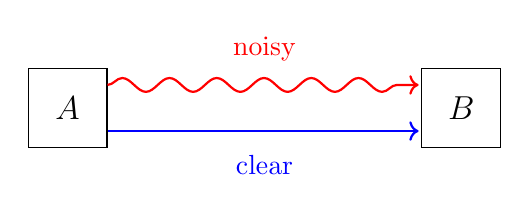
\begin{tikzpicture}[node distance=3cm]
            \node (a) at (3, 0) [rectangle, draw, font=\large, minimum size=1cm] {$A$};
            \node (b) at (8, 0) [rectangle, draw, font=\large, minimum size=1cm] {$B$};
            \draw [->, shorten > =0.1em, thick, red, decorate, decoration={
                segment length=6mm, snake, post length=1mm}]
                (a.30) -- (b.150)
                node [above=0.5em,align=center,midway] {noisy};

            \draw [->, shorten > =0.1em, thick, blue] (a.-30) -- (b.-150)
                node [below=0.5em,align=center,midway] {clear};
        \end{tikzpicture}
    \end{center}
    The noisy channel is a \hyperlink{def:bsc}{BSC} with error probability $p$.
    Bob chooses a \hyperlink{def:linearCode}{linear code} $C$ of length $d$, with suitable \hyperlink{def:weight}{weight} $d$.

    Alice chooses a linear map $\phi: C \to \F_2$.
    So, to send a bit $m \in \F_2$, Alice chooses a codeword $c \in C$ such that $\phi(c) = m$.
    She sends $c$ to Bob over the noisy channel, so $B$ receives $r \in \F_2^n$.
    Later Alice sends $c$ over clear channel.
    Bob checks $d(r, c) \approx n p.$.

    \begin{enumerate}[label=\arabic*)]
        \item Why can't Bob read the message? Since $C$ is chosen such that $d \ll np$, $B$ cannot recover $c$ from $r$.
        \item Why can't Alice cheat? She wants to substitute $c' \in C$ for $c$.
            She also knows $d(r,c) \approx np$, but does not know $r$.
            So she must cheat by using a $c'$ such that $d(r, c') \approx np$.
            But for $d$ large enough, since $c' \in C$, she has only one option - to send $c$.
    \end{enumerate}
\end{enumerate}

\subsection{Secret sharing via simultaneous linear equations}
Say there is a secret room that has an entry code $S \in \mathbb{N}$, known only to one person.
Say we also have a group of $n$ other people, who should be able to access the room, but only if $k$ or more of them are present.

How can we implement this? By Shamir, we get the system:
Suppose $0 < S < N$, and choose prime $p > N$.
Also, choose $a_1, a_2, \dotsc, a-{k-1}$, and distinct $x_1, \dotsc, x_n$ with $) \leq a_j \leq p-1$, $1 \leq x_j \leq p-1$ at random.
Also set $a_0 = S$, the key.
Define
\begin{equation*}
    P(r) = a_0 + \sum_{i=1}^{k-1} a_i x_r^i \pmod{p}.
\end{equation*}
We give the $r$th person the pair
\begin{equation*}
    (x_r, P(r))
\end{equation*}
called the shadow pair, which they keep secret. Everyone knows the prime $p$.
Suppose $k$ members are together with shadow pairs $(y_j, Q(j)) = (x_{r_j}, P(r_j))$ for $1 \leq j \leq k$.

By Van der Monde,
\begin{equation*}
    \det
    \begin{pmatrix}
        1 & y_1 & \dots & y_1^{k-1} \\
        1 & y_2 & \dots & y_1^{k-1} \\
        \vdots & \vdots & \ddots & \vdots \\
        1 & y_k & \dots & y_k^{k-1}
    \end{pmatrix}
    = \prod_{1 \leq i < j \leq k-1} (y_i - y_j)
    \not \equiv 0 \pmod{p}.
\end{equation*}
Thus can uniquely solve the system of $k$ equations
\begin{align*}
    z_0 + y_1 z_1 + y_1^2 z_2 + \dotsc + y_1^{k-1} z_{k-1} &\equiv Q(1) \pmod{p} \\
    \vdots \\
    z_0 + y_k z_1 + y_k^2 z_2 + \dotsc + y_k^{k-1} z_{k-1} &\equiv Q(k) \pmod{p}
\end{align*}
to get $z_0 = S$.

But for $k-1$ or fewer people, note by Van der Monde again for any value of $z_0$, the system gives solutions for $z_1, \dotsc, z_{k-1}$.
\end{document}
